\documentclass[letterpaper]{article}
\usepackage{cite}
\usepackage{amsfonts}
\usepackage{fancyhdr}
\usepackage[svgnames]{xcolor}
\usepackage[colorlinks=true,
            urlcolor=black!65!white,
            linkcolor=black!65!white,
            urlcolor=black!65!white,
            citecolor=black!65!white
            ]{hyperref}
\usepackage{url}
\usepackage{tikz}
\usetikzlibrary{shapes,snakes,arrows}
\usepackage{graphicx}
\usepackage{caption}
\usepackage{subcaption}
\usepackage{listings}
\usepackage[mono]{inconsolata}

\topmargin=-5mm
\evensidemargin=0cm
\oddsidemargin=0cm
\textwidth=16cm
\textheight=22cm
\addtolength{\headheight}{1.6pt}
\hypersetup{pdfstartview=}

\tikzset{>=latex}

\newcommand{\secref}[1]{\S\ref{#1}}
\newcommand{\lastupdate}{\today}
\newcommand{\ie}{\textit{i.e.}}
\newcommand{\mdash}{---}
\newcommand{\ecall}{\textsf{ecall}}
\newcommand{\ocall}{\textsf{ocall}}
\newcommand{\aex}{\textsf{AEX}}
\newcommand{\env}{\textsf{environment}}
\newcommand{\mrenclave}{\textsf{mrenclave}}
\newcommand{\mrsigner}{\textsf{mrsigner}}
\newcommand{\sha}{\textsf{sha256}}
\newcommand{\pve}{\textsf{PvE}}
\newcommand{\pce}{\textsf{PcE}}
\newcommand{\qe}{\textsf{QE}}
\newcommand{\launchenclave}{\textsf{Launch Enclave}}
\newcommand{\uc}{\textsf{UC}}
\newcommand{\se}{source-enclave}
\newcommand{\te}{target-enclave}
\newcommand{\rpk}{\textsf{Root Provisioning Key}}
\newcommand{\pk}{\textsf{Provisioning Key}}
\newcommand{\psk}{\textsf{Provisioning Seal Key}}
\newcommand{\rsk}{\textsf{Root Seal Key}}
\newcommand{\sk}{\textsf{Seal Key}}
\newcommand{\lk}{\textsf{Launch Key}}
\newcommand{\rk}{\textsf{Report Key}}

\title{\bf Intel SGX Remote Attestation is not sufficient}
\author{\textsc{Yogesh Prem Swami}}

\date{\lastupdate}

\begin{document}
\pagenumbering{arabic}

\maketitle

\begin{abstract}
  Intel SGX enclaves provide hardware enforced confidentiality and
  integrity guarantees for running pure computations (\ie, OS-level
  side-effect-free code) in the cloud environment. In addition, SGX
  remote attestation enables enclaves to prove that a claimed enclave
  is indeed running inside a genuine SGX hardware and not some
  (adversary controlled) SGX simulator.

  Since cryptographic protocols do not compose well
  \cite{cramerthesis,ucframework,gnuc}, especially when run
  concurrently, SGX remote attestation is only a necessary
  pre-condition for securely instantiating an enclave. In practice,
  one needs to analyze all the different interacting enclaves as a
  single protocol and make sure that no sub-computation of the
  protocol can be simulated outside of the enclave. In this paper we
  describe protocol design problems under (a) sequential-composition,
  (b) concurrent-composition, and (c) enclave state malleability that
  must be taken into account while designing new enclaves. We analyze
  Intel provided EPID \cite{epid} \textsf{Provisioning} and
  \textsf{Quoting} enclave \cite{sgxattest} within this framework and
  report our (largely positive) findings. We also provide details
  about SGX's use of EPID and report (largely negative) results about
  claimed anonymity guarantees.

\end{abstract}

\section{Introduction}
\label{sec:intro}
  Intel SGX enclaves\cite{sgxinnov, sgxinnov2} provide hardware
  enforced confidentiality and integrity guarantees for running pure
  computation (\textit{i.e.}, OS-level side-effect-free code) in the
  cloud environment. By limiting the application's Trusted Computing
  Base (TCB) to the CPU and CPU-Cache, SGX provides unprecedented
  confidentiality and integrity guarantees against malicious OS
  kernels and supervisor software. A popular design methodology---as
  evidenced by \cite{Haven, Graphene, Scone}---for creating secure
  cloud applications is as follows:

  \begin{description}
    \item[Step-1:] First, define a remote-attestation mechanism to
      securely instantiate an enclave. Quite often, this step is not
      explicitly stated probably because a generic black-box
      attestation scheme---whatever that means---is expected to be
      sufficient.
    \item[Step-2:] Then, largely independently of the
      remote-attestation mechanism, define the functionality that
      needs to be implemented inside the enclave. This step often
      involves composing different cryptographic as well as
      non-cryptographic protocols in ad-hoc ways to implement the
      desired algorithm. For example, the enclave may need to read
      encrypted keys from disk, compute a signature based on that key,
      create a new set of keys, etc.
    \item[Step-3:] Finally, define a ``run-time workflow," where one
      first validates the remote-attestation result, and then runs the
      algorithm implemented by the enclave. This step often requires
      multiple interactions with various other entities such as other
      enclaves, untrusted host software, trusted remote client
      software, and other cryptographic devices such as TPMs.
  \end{description}

  It's hard to argue against the simplicity and ease of implementation
  of such a modular software design. However, as pointed out in
  \cite{ucframework, cramerthesis}, unless a protocol is designed for
  ``\textsf{Universal Composition}" (\uc)---where, the real-world
  behavior and the ideal-world definition (function) of a protocol are
  computationally indistinguishable \textit{for every} adversary
  controlled environment---it's unlikely that arbitrary composition of
  such protocols will be secure. On the other hand, proving results in
  the \uc-framework is rather difficult. In this paper we propose a
  framework for analyzing SGX enclaves that's a compromise between a
  full \uc-based analysis and completely ad-hoc composition. Before
  describing the framework, we illustrate the problem associated with
  the protocol composition with two real-world examples.

  To set the stage, a cloud service provider wanted to migrate its new
  clients from Amazon Cloud-HSM to an SGX enclave. The protocol for
  interacting with the enclave was based on HTTP Request/Response
  framework, where different operations (such as \textsf{KeyGen}),
  were sent as a command, and the enclave would execute and return a
  response (including explicit error codes) back to the remote caller.
  Important use-case for the enclave were to support (a) local key
  generation, (b) storing the public/private key on disk with an AEAD
  scheme that would allow \textit{fast} key look-up, and (c) creating
  Certificate Signing Requests (CSR) from the enclave using
  challenge-response protocol \cite[\S5.2.8.3]{rfc4210}, among other
  things. Figure~\ref{fig:sequentialcomp} describes one execution path
  of the protocol.

  \begin{figure}[h]
  \centering
  \begin{subfigure}[b]{.5\textwidth}
    \centering
    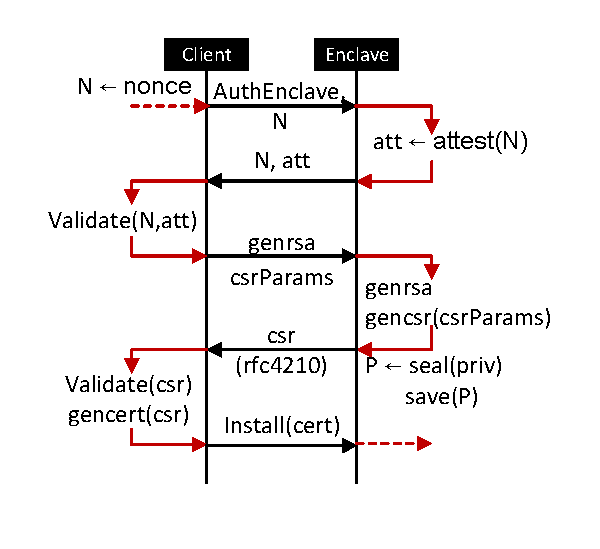
\includegraphics[width=.95\linewidth]{Diagrams/SeqCompProblem}
    \caption{Command execution for \textsf{KeyGen} with Cert}
    \label{fig:sequentialcomp}
  \end{subfigure}%
  \begin{subfigure}[b]{.5\textwidth}
    \centering
    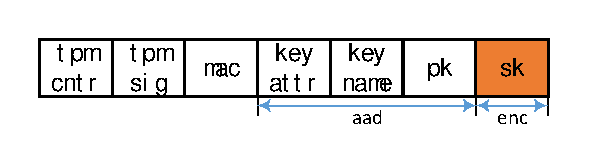
\includegraphics[width=.95\linewidth]{Diagrams/MsgFmt}\\\vfill
    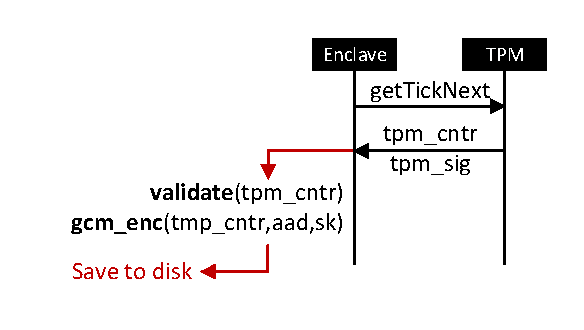
\includegraphics[width=.95\linewidth]{Diagrams/SealProtocol}
    \caption{Message format and seal protocol}
    \label{fig:sealprotocol}
  \end{subfigure}
  \caption{Example of a flawed key-management enclave. The command
    execution protocol ascertains the authenticity of the enclave by
    validating the EPID signature on a randomly generated 256-bit
    nonce, followed by executing an arbitrary mix of commands as
    required by the use-case. Long-term keys are stored as
    GCM-encrypted AEAD blobs. The nonce (a 32-bit counter zero-padded
    on the left to 96-bit) for each GCM record is stored in TPM, and
    the TPM returns a signature on the nonce (along with some
    additional data---to disable roll-back of TPM ``ticks.'' The
    enclave validates the TPM's signature before using the nonce for
    sealing.}
  \label{fig:usecase}
  \end{figure}

  This seemingly secure protocol is, in fact, not secure at
  all. Notice that the remote attestation in
  Figure~\ref{fig:sequentialcomp} does not prevent a malicious cloud
  service provider from first faithfully responding to remote
  attestation queries, but then emulate the rest of the protocol
  (including \textsf{KeyGen} and CSR) outside of the enclave. While
  this is obvious in this simplified example, in a more complicated
  scenario, where multiple enclaves are interacting with each other,
  it might not be obvious if certain sub-components of the protocol
  can be simulated outside. Even though the entire enclave is
  \textit{sequentially composed} from potentially provably-secure
  protocols, the combined protocol is completely insecure.

  Second, consider the seal protocol. Here each record (see
  Figure~\ref{fig:sealprotocol}) is GCM-encrypted using a nonce
  generated and signed by a TPM. However, consider a cloud service
  provider who instantiates two copies of the same enclave and
  \textit{concurrently} executes \textsf{KeyGen} using the same TPM
  signed counter. In this case, each enclave will generate two
  different keys in response to \textsf{KeyGen}. However, since the
  two concurrent instances will each correctly verify the signature
  (the two enclaves are identical), each will end up using the same
  nonce with different underlying data! As is the case with all
  counter modes, reusing the nonce can completely destroy the security
  of the system\footnote{In the present case, since the underlying
    data is uniformly distributed, at least for AES or ECDSA keys,
    such a concurrent composition might not be harmful. However, if
    there is even a small bias in the random number generator, it
    might be possible to build a distinguisher from the \texttt{xor}
    of cipher-text data.}. Note that this is not a flaw in GCM or in
  the way the TPM is used\footnote{When using TPMs with SGX enclaves,
    it's important that both the TPM and the enclave mutually
    authenticate each other. Failure to do so can lead to replay
    attacks where the adversary swaps the motherboard and in doing so
    resets the TPM counter. In the present case, however, even
    mutually authenticated TPM counter might not be secure under
    concurrent composition.}, rather, it's a case where an otherwise
  secure protocol is insecure under concurrent composition.

  While these examples describe a totally broken scheme, in practice
  sequential and concurrent composition may not completely break the
  system as above. Rather it might just weaken the \textit{bounds} of
  the entire protocol making it easy for further crypt-analysis. For
  example, consider a scheme that consists of to two protocols $\pi_1$
  and $\pi_2$, where the adversary needs $2^{t_1}$ and $2^{t_2}$
  oracle queries to break $\pi_1$ and $\pi_2$ respectively. However,
  its possible that when composed sequentially as $(\pi_1 \circ
  \pi_2)$ or $(\pi_2 \circ \pi_1)$ the number of queries needed to
  break the composed protocol is smaller than
  $2^{\min\{t_1,t_2\}}$. In fact, since protocol composition rarely
  commutes, even different order of composition might result in very
  different bounds\footnote{Readers familiar with
    \textsf{encrypt-then-mac} vs.  \textsf{mac-then-encrypt} debate
    should require no further explanation.}.
  
  To summarize, \textit{an enclave is a protocol} composed of several
  sub-protocols. In order for the enclave to be secure, it's essential
  that sequential and concurrent composition of sub-protocols remain
  secure. The rest of this document is organized as follows.
  \secref{sec:model} describes the abstract computational model of SGX
  that's better suited for security analysis. \secref{sec:analysisfwk}
  describes pitfalls of sequential, concurrent, and parallel
  composition of cryptographic protocols and describes ways in which
  an enclave can be abused by a malicious cloud service
  provider. \secref{sec:remoteatt} describes Intel's remote
  attestation framework, and describes in detail the SGX remote
  attestation mechanism.

  \section{SGX Computational Model}
  \label{sec:model}
  Intel documentation\cite{intelsdm} provides excellent low-level
  details about the SGX instructions. This section provides an
  abstract computational model of SGX which is better suited for
  security analysis.

  Abstractly, an SGX enclave can be thought of as a black-box that's
  capable of running any arbitrary algorithm. The black-box (enclave)
  can communicate with the outside world, called the \env, in three
  different ways:

  \begin{figure}[h]
  \centering 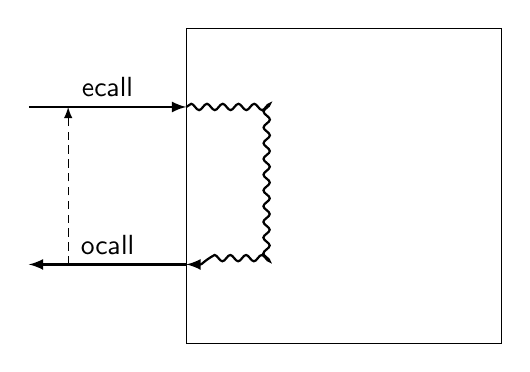
\begin{tikzpicture}[x=1cm, y=-1cm]
  \newcommand{\ench}{4cm}
  \newcommand{\encw}{4cm}
  \newcommand{\alen}{1cm}
  \newcommand{\adiff}{1cm}

  \node[rectangle, minimum height=\ench, minimum width=\encw, draw] (enc) {};
  \draw[->,thick] (-\encw / 2.0 - 2*\alen, \adiff ) -- (-\encw/2.0, \adiff) %%
  node [midway, above] {\textsf{ecall}};

  \draw [->, thick, decorate, %%
    decoration={snake,amplitude=.4mm,segment length=2mm, post length=1mm}] %%
  (-\encw/2.0, \adiff) -- (-\encw/2.0 + 1*\adiff + 0.1, \adiff) -- %%
  (-\encw/2.0 + 1*\adiff , -\adiff) -- (-\encw/2.0, -\adiff);


  \draw[<-,thick] (-\encw / 2.0 - 2*\alen, -\adiff ) -- (-\encw/2.0, -\adiff) %%
  node [midway, above] {\textsf{ocall}};

  \draw[->, thin,densely dashed] (-\encw / 2.0 - 1.5*\alen, -\adiff ) -- %%
  (-\encw/2.0 - 1.5*\alen , \adiff);
\end{tikzpicture}

  \caption{SGX Computational Model.}
  \label{fig:model}
  \end{figure}

  \begin{description}
  \item[\ecall:] The \env\ can invoke a pre-defined function inside
    the enclave by passing input parameters and returning internal
    state of the enclave as results. Such invocations from the
    \env\ to the enclave are referred to as \ecall. The parameter
    values passed from the \env\ to the enclave are either copied or
    directly shared with the enclave. An \ecall\ can terminate in one
    of the three ways: (a) by returning normally as a function from
    the enclave, (b) by making an explicit \ocall, or (c) as the
    result of an interrupt or exception.

    SGX also supports multi-threading, and it's possible for the
    \env\ to run the same \ecall\ in different threads. However, once
    an \ecall\ has acquired the thread, future attempts to reuse that
    same thread will result in error. Further more, the number of
    threads that an enclave can support is pre-determined by the
    enclave signer, and cannot be altered at runtime.

  \item [\ocall:] While an enclave is executing (because of some
    previous \ecall), it can make \ocall s to pre-designated functions
    in the \env.  Unlike an \ecall, an \ocall\ cannot directly share
    the internal enclave state with the \env, and must---directly or
    indirectly---copy the parameters into the \env\ before making an
    \ocall.

    An interesting characteristic of an \ocall\ is that the \env\ is
    not required to return back to the enclave at the end of the
    \ocall\ (see Figure~\ref{fig:model}). Since the behavior of
    pre-designated functions in the \env\ are controlled by the
    adversary, one should not expect the \env\ to follow the protocol
    that enclave author had envisioned. In particular, it's possible
    to create a chain of \ecall s and \ocall s such that the adversary
    can perform operations on the internal (global) state of the
    enclave. We call such adversarial manipulation of internal enclave
    state as \textit{enclave malleability}.

  \item[\textsf{Asynchronous Exit}:] In addition to an \ocall, the
    processor can exit from an enclave due to an interrupt or
    exception. Such enclave exiting events are called
    \textsf{Asynchronous Exit Events}, or \aex. Unlike an \ocall, an
    \aex\ can transfer control from the enclave to the \env\ at
    arbitrary (possibly adversary controlled) points inside the
    enclave. Like \ocall s, an \aex\ can either by resumed from where
    the enclave left off, or the environment can invoke another
    \ecall\ (either within the same thread or a different thread).

    Since an adversary can create multiple running copies of an
    enclave and selectively interrupt each enclave to cause and \aex,
    it can be used as a means to ``rewind'' the internal state of the
    enclave. Given that proof-of-knowledge \cite{BellarePOK} protocols
    fundamentally have a \textit{knowledge-extractor} based on
    rewinding, an enclave must ensure that it does not leak secrets
    when interrupted by an \aex.

  \end{description}

  \subsection{Enclave Creation}
  \label{sec:enclavecreateion}
  An enclave is generated as a dynamically shared library using
  standard compiler tools. In addition, the entity creating the
  enclave must also decide up-front on the following information:

  \begin{description}
  \item[\textsf{Attributes}:] The attributes of an enclave act as an
    access control mechanism that is enforced by the hardware. For
    example, certain high privilege keys, such as \lk\ and
    \textsf{Provisioning Key}, cannot be made accessible to all the
    enclaves, as it would compromise the security of entire SGX
    ecosystem. In order to gain access to these keys, an enclave
    author must explicitly request for these attributes at
    compile/sign time. During enclave launch-time, the \launchenclave,
    based on policy decisions, decides whether to grant or reject
    requests based on these attributes.

  \item[\textsf{Stack size}:] The enclave author must estimate the
    size of the stack needed by the enclave and set its value at
    enclave creation time. Once an enclave is instantiated, this value
    cannot be changed.

  \item[\textsf{Heap size}:] Like the stack size, the heap-size of the
    enclave is also fixed at enclave creation time. In SGXv2, this
    value can be changed post-instantiation.

  \item[\textsf{Thread count}:] An enclave must also decide upon the
    number of threads that can run concurrently. As pointed out in
    \secref{sec:model}, concurrency can have a dramatically negative
    impact on the security of the certain protocols, and one must not
    select this parameter just on the basis of performance
    requirements, but also on the basis of security concerns.

  \item[\textsf{Software version}:] SGX provides elaborate
    software-upgrade and life-cycle management facilities and allows
    software vendors to make use of these features.

  \end{description}

  Based on these parameters, the enclave signing tool creates a
  virtual memory layout of the enclave and computes a hash of the
  entire memory layout (including the stack, heap, thread control
  structure, etc.)  See \cite{intelsdm} for details about how the hash
  is computed. This hash, called \mrenclave, is used as the unique
  identifier for the enclave.

  In addition to \mrenclave, the software vendor must also sign the
  enclave using a RSA-3072 key. The hash of the RSA Public-Key is
  called \mrsigner. As described in \cite{surnaming}, the purpose of
  the signature is to provide an unforgeable identity---a
  \textit{surname} based lineage---to a set of enclaves based on the
  vendor.

  It should be noted that the \mrenclave\ of an enclave doesn't change
  even when the signing key is changed. This is significant when
  validating attestation or deriving keys based on \mrenclave.

  \subsection{Enclave instantiation and access control}

  A properly signed enclave can be instantiated on any Intel SGX
  Processor---subject to access control restrictions enforced by
  \launchenclave. Before an enclave can be instantiated on an SGX
  capable processor, it must get an authorization token, called
  \textsf{Launch Token}, from Intel provided \launchenclave. The
  \launchenclave\ uses a combination of \mrenclave, \mrsigner, the
  attributes of the enclave and a \textit{white-list signed by Intel}
  to decide whether to grant \textsf{Launch Token} to the enclave or
  not. Once an enclave obtains a \textsf{Launch Token}, the enclave
  can continue using it indefinitely, even when the policies of the
  \launchenclave\ might get updated later on.

  \subsection{SGX Platform Keys}
  \label{ssec:platkeys}

  As described in \cite{sgxattest}, each Intel SGX capable processor
  contains two statistically independent base keys: \rpk\ and \rsk.
  The \rpk\ is used as the \textit{root-of-trust} between the CPU and
  Intel Attestation Services (IAS) \cite{ias}. Intel retains a copy of
  this key at the time of manufacturing and uses it to establish the
  trustworthiness of the processor during EPID join process. Intel
  claims that \rsk\ is not retained. However, it's not clear whether
  this key is generated inside the processor via oracle access (\ie,
  in such a way that CPU generates the key all by itself using it's
  own internal random numbers or with PUFs), or whether the key is
  first generated outside the processor, then injected into CPU, and
  finally all outside references destroyed. Unless these keys are
  generated via oracle access, one should consider \rsk\ to be known
  to Intel.

  \begin{figure}
  \centering
  \begin{subfigure}[t]{.45\textwidth}
    \centering
    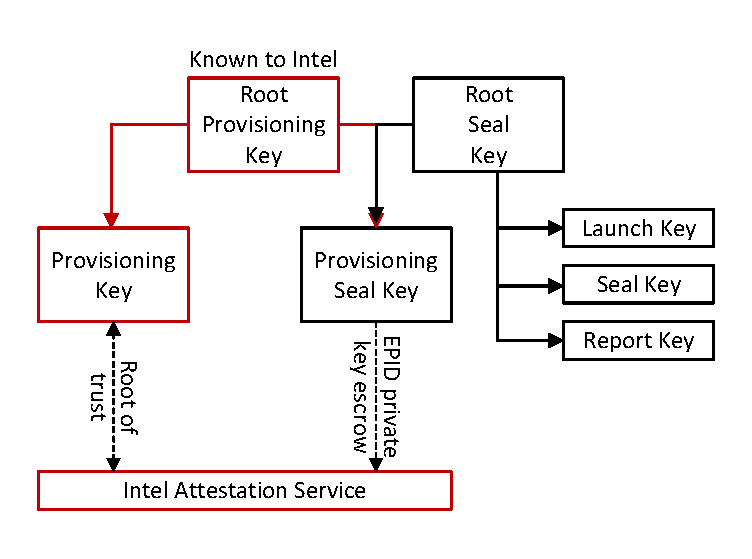
\includegraphics[width=\linewidth]{Diagrams/KeyHierarchy}
    \caption{The \pk\ acts as a root-of-trust between SGX capable CPU
      and Intel Attestation Service. \psk\ is used for EPID private
      key escrow.}
    \label{fig:keyhierarchy}
  \end{subfigure}
  \hspace{.05\textwidth}
  \begin{subfigure}[t]{.45\textwidth}
    \centering 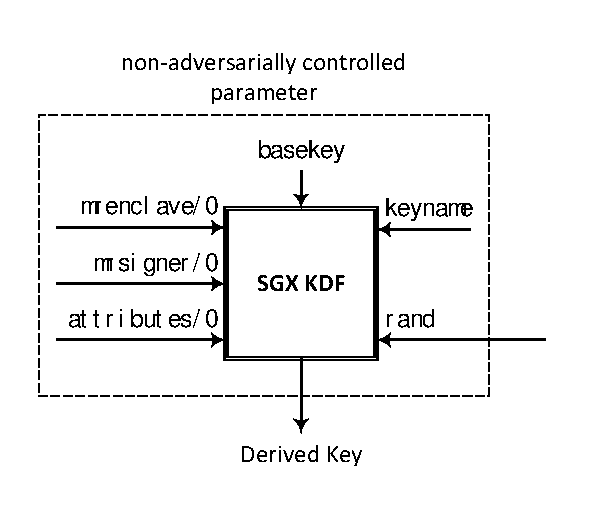
\includegraphics[width=\linewidth]{Diagrams/SGXKDF}
    \caption{SGX Key derivation function. Only parameters outside the
      dotted line can be chosen maliciously. Key derivation uses
      all-zeros for \mrenclave, \mrsigner, and attributes if key
      policy doesn't specify which ones to use. See
      \cite[\S38.17]{intelsdm} for additional details.}
    \label{fig:sgxkdf}
  \end{subfigure}
  \caption{SGX Platform and Named Key.}
  \label{fig:keys}
  \end{figure}

  An application software does not have raw access to these base
  keys. However, an application can access \textit{named} keys that
  are derived from these two base key (see Figure~\ref{fig:keys}).
  The key derivation function allows enclave author to specify
  policies on how to derive enclave specific keys from base
  keys. These policies allow enclaves to use the \mrenclave,
  \mrsigner\ and/or attributes from the trusted CPU cache to derive
  keys. An implication of this design is that enclaves cannot derive
  keys that might belong to a different enclave. Also note that when
  key derivation policy does not require specific field such as
  \mrenclave\ to be used, a default value of all-zeros is
  used. Therefore, even when ``raw'' named keys are available that
  have not been specialized for any particular enclave, it's not
  possible to derive specialized keys from the raw key. For example,
  one can obtain the raw \sk\ that is neither tied to \mrenclave\ or
  \mrsigner\ of any enclave, and yet it's not possible to derive
  enclave-specific \sk\ from the raw \sk.

  The following list describes user accessible keys and their intended
  usage:

  \begin{description}
  \item[\pk:] This key is derived from \rpk\ and is used as a software
    version dependent root-of-trust between Intel Attestation Service
    and SGX capable processor. Since admitting a non-SGX processor to
    the Intel Attestation Service's group of SGX processors will
    completely compromise remote attestation for all CPUs, extreme
    care must be taken in granting access to Provisioning
    Key. Currently, the \launchenclave\ only grants Provisioning Key
    access to enclaves that have been signed by Intel. Furthermore,
    only \textsf{Provisioning Enclave} (\pve) and Provisioning
    Certification Enclave (\pce) (both created without debug option)
    have access to this key.

  \item[\psk:] This key is derived jointly from Root Provisioning Key
    and Root Seal Key. During the EPID join process, the EPID
    private-key for each platform is encrypted with this key and
    uploaded to Intel Attestation Service. (See \secref{ssec:epidprov}
    for details about EPID join process.)

    Note that the EPID private-key could not just be encrypted with
    \pk\ as that would destroy the EPID's blinded-join
    protocol. Conversely, the EPID private-key cannot be encrypted
    just with \sk\ as that might allow non-privileged enclaves to have
    access to EPID private key and thereby render Remote Attestation
    ineffective.

    In spite of this design choice, given the uncertainty about how
    the \rsk\ is generated, one should assume that Intel knows the
    EPID private key for each platform.

  \item[\lk:] This key is derived from \rsk\ and is used by
    \launchenclave\ to create authorization tokens
    (\textsf{EINITTOKEN}) that each non-Intel enclave must obtain in
    order to instantiate an enclave. Only a specific \mrsigner---whose
    corresponding private-keys are only known to Intel---can access
    the \lk. In SGXv2, the \mrsigner\ for \launchenclave\ can be
    changed pragmatically, (see \cite[\S39.1.4]{intelsdm}) but it's
    not clear how Intel intends to enforce access control restrictions
    on \pk.

  \item[\sk:] This key is derived from \rsk\ and used for encrypting
    data specifically for a given CPU.

  \item[\rk:] This key is derived from \rsk\ and used for Local
    Attestation (see \secref{ssec:localatt} for detailed information
    on Local Attestation and how Report Key is used).

  \end{description}

  \subsection{Local Attestation}
  \label{ssec:localatt}

  \begin{figure}
    \centering
    \begin{subfigure}[h]{.5\textwidth}
      \centering
      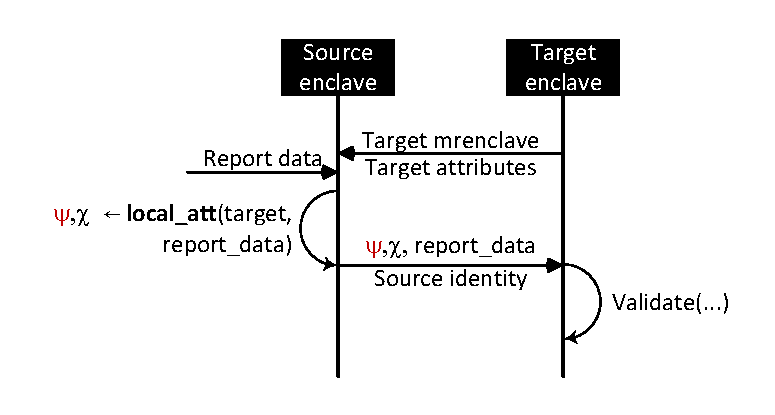
\includegraphics[width=.95\linewidth]{Diagrams/LocalAttestationFlow}
      \caption{Local attestation message flow.}
      \label{fig:localattestationflow}
    \end{subfigure}%
    \begin{subfigure}[h]{.5\textwidth}
      \centering
      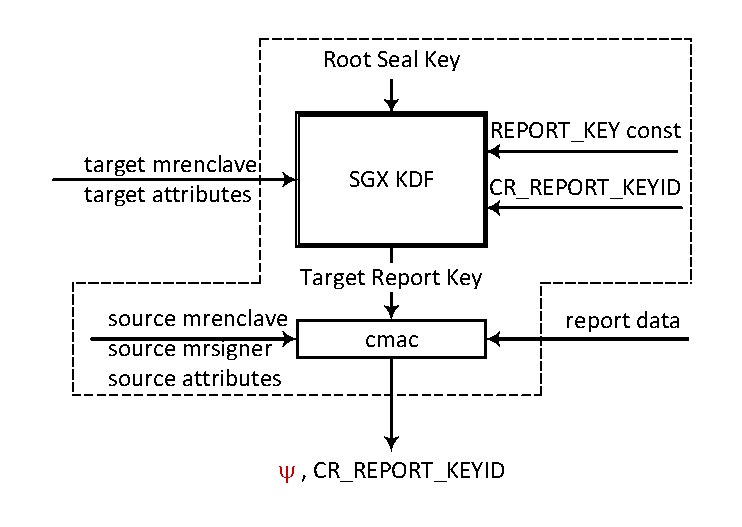
\includegraphics[width=.85\linewidth]{Diagrams/LocalAttestation}
      \caption{Local attestation computation. Parameters outside the
        dotted line can be adversarialy selected.}
      \label{fig:localattestation}
    \end{subfigure}%
    \caption{Local attestation computation and message flow}
    \label{fig:localatt}
  \end{figure}

  The process of local-attestation allows a source enclave (\se) to
  prove to a target enclave (\te)---running locally on the same
  platform---that the \se\ is indeed running on a genuine Intel SGX
  platform (see Figure~\ref{fig:localattestationflow}). In addition,
  the \se\ can optionally use 512-bits of additional data (e.g., hash
  of public-key), called report-data, to claim knowledge of certain
  bit-string.

  The process of local-attestation involves computing CMAC
  \cite{aescmac} on the \se's identity (i.e., \mrenclave, \mrsigner,
  etc.) using the \te's Report Key. However, as pointed out in
  \secref{ssec:platkeys}, the \se\ cannot directly access \te's Report
  Key. SGX solves this problem by providing \textit{oracle access} to
  \te's Report Key via \textsf{EREPORT} instruction
  \cite[\S14.4.1]{intelsdm}.
  
  To compute local attestation, the \se\ obtains the \mrenclave\ and
  attributes of the \te\ through some out-of-band mechanism (which
  might be adversarial). Based on \te's \mrenclave, the
  \textsf{EREPORT} instruction internally derives the \te's Report Key
  and computes \textsf{CMAC} on \se's \mrenclave, \mrsigner, and
  attributes from the trusted CPU cache (and optionally untrusted user
  data).  The \textsf{EREPORT} instruction also uses a boot-time
  random number called \textsf{CR\_REPORT\_KEYID} to diversify the
  \te's Report Key before \textsf{CMAC} computation. The
  \textsf{EREPORT} instruction also returns the value of
  \textsf{CR\_REPORT\_KEYID} that was used during \te's Report Key
  derivation.

  The verification of local attestation involves using
  \textsf{EGETKEY} instruction to fetch the \te's Report Key and
  validating the \textsf{CMAC} on Report body in software.  The report
  body includes \mrsigner, \mrenclave, attributes, and other
  parameters of the \se. Note that while fetching the \rk\ for
  verification, the \textsf{EGETKEY} will require the value of
  \textsf{CR\_REPORT\_KEYID} to derive the right \rk.

  \section{Enclave malleability and Knowledge Extractors}
  \label{sec:analysisfwk}

  Given the computational model of SGX, we describe certain pitfalls
  in enclave design that might inadvertently make the enclave
  malleable, or open door for building knowledge-extractors
  \cite{BellarePOK}.

  \subsection{Enclave malleability}
  \label{ssec:malleability}
  As described in \secref{sec:model}, an application can exit an
  enclave either via (a) as a function return from an \ecall\ (b) as
  an \ocall\ or (b) as an \aex. Since it's not required for an
  \ocall\ or \aex\ to return back to the enclave from the state it
  left off, it's possible for a malicious \env\ to make unexpected
  \ecall s to alter the internal state of the enclave. Enclaves whose
  global internal state can be influenced by an attacker by not
  following the expected protocol are called \textit{malleable
    enclaves} in this document.

  To better understand enclave malleability, consider the following
  example: The US government wants to use an SGX enclave to implement
  2-man rule for launching nuclear missiles. The 2-man rule requires
  that at least two \textit{different} members (generals) of the armed
  forces authorize the launch a nuclear missile.

  Listing~\ref{code:malleability} describes one way to implement this.
  Essentially, the enclave keeps a list of generals, their
  public-keys, and their individual authorization state in a global
  variable \texttt{GENERALS}. In addition, the enclave keeps the
  number of distinct generals who have authorized the launch in a
  global variable \texttt{auth\_count}. Since different generals might
  be authorizing the launch at different times, the enclave allows
  each general to authorize a launch individually by signing the
  concatenation of general's name and some auxiliary data.

  \begin{center}
  \lstset{language=C++, numbers=left, numberstyle=\tiny,
    numbersep=5pt, stepnumber=1, emph={auth_and_launch,auth_count},
    emphstyle=\color{red!80!black}, emph={[2]valid_general},
    emphstyle={[2]\color{green!40!black}}, basicstyle=\ttfamily,
    keywordstyle=\color{blue}\ttfamily,
    stringstyle=\color{red}\ttfamily,
    commentstyle=\color{brown}\ttfamily,
    morecomment=[l][\color{magenta}]{\#} }
  \begin{lstlisting}[captionpos=b,
                     caption={An enclave suseptible to state
                       malleability}, label=code:malleability] 
/* count of generals who have authorized launch. */ 
static int auth_count = 0;

/* hardcoded list of generals and their PKs */ 
struct general_info{
  char general_name[256]; 
  const sgx_ec256_public_t general_pub; 
  bool has_authorized; // initialized to false 
}GENERALS[] = { ... };

/* ecall made by each general with a sig on name + aux data */ 
int auth_and_launch(const char* const general_name, 
                    const sgx_ec256_signature_t* sig){ 

  struct general_info* valid_general = 
          validate_general(general_name, sig);

  if(!valid_general){ return INVALID_GENERAL; }

  if(!valid_general->has_authorized){ 
    auth_count++; // AES here will be devastating!  
    valid_general->has_authorized = true; 
  }else{
    return GENERAL_ALREADY_AUTHORIZED_ACTION; // replay 
  }

  if(auth_count == 2){ 
    return nuke_the_kashbah(location); 
  }

  return PENDING_AUTHORIZATION; 
}
\end{lstlisting}
\end{center}

  Can this enclave be exploited to launch a missile with \textit{just
    one} authorization, say $\langle g_1, \sigma_1 \rangle$?
  Surprisingly, the answer is yes! Here is how:

  \begin{enumerate}
  \item The attacker first feeds $\langle g_1, \sigma_1 \rangle$ to
    \texttt{auth\_and\_launch} function with the intent of causing an
    \aex\ between lines 19 and 20. Since the attacker can artificially
    cause an interrupt and also instantiate multiple copies of the
    enclave in parallel, given a polynomial number of trials (in
    program length), the attacker can cause an \aex\ between line 19
    and 20 W.H.P. Note that at the time of a successful \aex\ between
    line 19 and 20, the \texttt{auth\_count} and
    \texttt{has\_authorized} variables will be in an inconsistent
    state where the \texttt{has\_authorized} would still be
    \texttt{false} and another \ecall\ to \texttt{auth\_and\_launch}
    will successfully update the \texttt{auth\_count} variable.

  \item After the enclave has been interrupted by \aex\ and the
    processor is ready to resume, the attacker instead of resuming,
    makes an \ecall\ to \texttt{auth\_and\_launch} again with the same
    old parameters $\langle g_1, \sigma_1 \rangle$. Since the first
    \ecall\ had incremented the counter, but left the authorization
    state inconsistent, the second \ecall\ will once again increment
    \texttt{auth\_count} leading to a nuclear attack!

  \item While not applicable in this case, in some cases it might be
    necessary for an attacker to resume the first \ecall\ after the
    second one has completed. Since the enclave preserves the stack
    before making an \aex, resuming the first \ecall\ tantamounts to
    executing \textsf{ERESUME} assembly instruction.

  \end{enumerate}

  It should be emphasized that the problem of state-malleability,
  where the attacker can influence the internal state of the enclave
  without ever having direct authorized access to it, is broader in
  scope than the race condition described above. For example, one can
  use malleability to induce an error which turns the enclave into an
  oracle. It should also be emphasized that enclaves should return
  error codes with security consideration in mind.

  \subsection{Enclave rewinding and knowledge-extractors}
  \label{ssec:rewind}

  Zero-Knowledge Proof of Knowledge (ZKPK) protocols, by definition
  have in-built knowledge-extractor \cite{BellarePOK, maurerZKP}.
  Normally, the knowledge-extractor from the prover is designed by
  giving a simulator the capability to ``rewind'' the prover's state
  to arbitrary point during it's execution. Since SGX enclaves can be
  interrupted by an \aex, it's important that a malicious \env\ is not
  able to rewind the enclave in such a way that it inadvertently
  reveals the secret-key.

  Consider the three-move---commit, challenge,
  blinded-reveal---$\Sigma$-protocols \cite{sigmaprotocol} that are
  the most efficient and widely-used ZKPKs protocol in practice.
  Normally, one designs $\Sigma$-protocols \textit{with interaction}
  between a prover and a verifier in mind, and then uses Fiat-Shamir
  \cite{FiatShamir} heuristic\footnote{In the Fiat-Shamir heuristic,
    the prover \textit{pretends} to be a verifier and a random oracle,
    based on publicly known fields of the protocol (such as the
    commitment value, user's input message, etc.) generates the
    challenge string.} to convert it into a useful non-interactive
  use-case such as a signature scheme. Most of these protocols just
  require the prover, which in this case will be enclave, to respond
  to two challenge message for a given commitment message to reveal
  the secret.

  If an enclave is not implemented appropriately, one can induce an
  artificial \aex\ right after the commitment phase, and call the
  enclave with different messages in possibly different threads to
  generate two responses to the same commitment message. Note that
  \aex in conjunction with multi-threading opens doors for a limited
  form of enclave rewinding and presents a larger attack surface than
  \aex alone.  Unless, an enclave requires multi-threading, it's wise
  to set the number of possible threads to the bare minimum.

  \section{SGX remote attestation}
  \label{sec:remoteatt}

  SGX is an example of a hardware/software co-design of a
  cryptographic platform. A common concern in the design of such
  systems is to ensure that an adversary is not able to switch the
  hardware with a software simulator (such as QEMU \cite{qemu,
    opensgx}) of the hardware. Since an Universal Turing Machine can
  simulate any piece of computing hardware, unless there's an inbuilt
  asymmetry between what the software ``knows'' and what the hardware
  knows, it's impossible to prevent software simulator attacks in such
  systems. On the other hand, each independent piece of software needs
  to prove on its own that it's running on a real hardware.
  Therefore, each independent software must somehow have direct or
  oracle access to the secret that the hardware is holding. The
  essence of any remote-attestation scheme in such systems is to
  address these two conflicting requirements. {\em Note}: Even
  limiting access to raw hardware keys via an oracle is not sufficient
  to thwart simulator based attacks. An attacker can run it's hardware
  simulator on a real hardware, gain access to the hardware-secret via
  the oracle, and then impersonate as the real hardware.

  In case of Intel SGX, the question of knowledge-asymmetry between
  hardware and software is answered by the \rpk\ (see
  \secref{ssec:platkeys}). The dilemma of both denying as well as
  granting access to this hardware secret is solved by a two-step
  process:

  \begin{enumerate}
    \item Intel has created a (set of) privileged enclaves---called
      \textsf{Provisioning Enclave} (\pve) and \textsf{Provisioning
        Certification Enclave} (\pce)\footnote{Intel addresses these
        enclaves by their acronyms, \pve\ and \pce, only. The
        descriptive names are author's interpretation.}---with raw
      access to the Provisioning Key and Provisioning Seal Key. The
      \pve\ and \pce\ use the Provisioning Key as the root-of-trust
      between Intel Attestation Service and the SGX CPU to bootstrap a
      new set of credentials for a Group Signature Scheme called
      Enhanced Privacy ID (EPID) \cite{epid}. Since EPID key
      provisioning takes place only once\footnote{EPID re-provisioning
        might take place if the CPU's Security Version Number (CSVN
        \cite[\S39.4.2.2]{intelsdm}) or the Software Version Number
        (ISVSVN \cite[\S39.4.2.1]{intelsdm}) of \pce\ changes.}, the
      Provisioning Key has minimal exposure.

    \item Once a platform has been provisioned with EPID keys, another
      Intel signed enclave called \textsf{Quoting Enclave} (\qe) is
      given raw access to EPID keys and made responsible for
      generating remote-attestation results on behalf of other
      arbitrary--potentially malicious---enclaves.

      To compute remote attestation, an arbitrary enclave first
      generates a local attestation with \textsf{Quoting Enclave} as
      the target enclave in Figure~\ref{fig:localattestationflow}. The
      \textsf{Quoting Enclave} first validates the local-attestation
      report and subsequently uses EPID key to sign all the parameters
      it validated during local attestation. Since local-attestation
      uses the hardware resident identity of the enclave (i.e.,
      \mrenclave, \mrsigner, and enclave attributes), which cannot be
      forged (see \secref{ssec:localatt}), the remote-attestation
      result on the enclave identity cannot be forged
      either. Furthermore, since arbitrary software never has direct
      or oracle access to either Provisioning Key or EPID
      private-keys, simulator based attacks where the simulator itself
      is a valid enclave are also thwarted.
  \end{enumerate}

  The rest of this section is organized as follows: \secref{ssec:epid}
  provides an overview of EPID and how it's has been implemented by
  Intel. Since the official \cite{epid} paper leaves several details
  out (e.g., the Zero-Knowledge proof of inequality for signature
  based revocation is left out from the paper), the goal of this
  section to fill in those gaps based on \textsf{Provisioning Enclave}
  and \texttt{epid-sdk} open source implementation
  \cite{epidsdk}. \secref{ssec:epidprov} provides detailed information
  on how the \textsf{Provisioning Enclave} joins the SGX EPID
  group. Finally, \secref{ssec:qe} provides details about
  \textsf{Quoting Enclave} and how SGX remote attestation should be
  validated against Intel Attestation Service.

  \subsection{EPID Overview}
  \label{ssec:epid}
  In a standard signature scheme, such as ECDSA or RSA-PSS, each
  signer has a unique private/public key-pair. Given two
  message/signature pairs $\langle m_1, \sigma_1 \rangle$ and $\langle
  m_2, \sigma_2 \rangle$, an attacker in possession of $N$ public-keys
  can easily determine if $m_1$ and $m_2$ were signed by the same
  private key or not. If such signatures are generated by physical
  devices, it can be used to track the signing device and thereby
  destroy the anonymity and privacy of the person using that device.

  Group Signatures were introduced by Chaum and Van Heyst
  \cite{ChaumGroupSignatures} as a means to address this. Their idea
  was to create a signature-scheme where a single ``group
  public-key,'' can verify messages signed by different private
  keys. In addition to anonymity, several additional requirements were
  later on added to this list to different use cases.

  The literature on group signature schemes is huge, both for formal
  models of its security
  \cite{BMW03,dynamicGroupSignatures,fulldynamicgroupsignature} as
  well as for different constructions \cite{bbs, Furukawa2005,
    coalitionresistant, camenischLysyankaya} based on different
  computational assumptions. From a practical deployment perspective,
  Direct Anonymous Attestation \cite{daa, ucdaa} (DAA) is closest to
  EPID and also most widely deployed.


  In EPID, there are four entities:

  \begin{description}
  \item [Issuer ($\mathcal{I}$):] It's the entity that decides who
    should be part of a given EPID group. In case of SGX, the Intel
    Attestation Service acts as the issuer. Its goal is to dynamically
    (i.e., one-by-one) add new SGX Processors as they come
    on-line. Group signature schemes do no define what credentials one
    must possess before they can be admitted to given group. However,
    for group signatures to be meaningful, some form of out-of-band
    mechanism must decide group membership criteria. In case of SGX,
    the Intel Attestation Service uses knowledge of Root Provisioning
    Key as the deciding factor on who should join the SGX Processor
    group (see \secref{ssec:epidprov}).

  \item[Revocation Manager ($\mathcal{R}$):] Unlike standard signature
    schemes, where revocation only includes the public-key of the
    revoked private-key, group signatures require a different
    approach. EPID has two forms of revocation:

    \begin{itemize}
    \item Private-key based revocation list, called \texttt{Priv-RL},
      which is a list of all the compromised \textit{private-keys}
      known to Revocation Manager. EPID does not support
      full-anonymity\footnote{In the \textsf{anonymity} game of
        \cite{BMW03}, the adversary gets the private key of all the
        members, and yet cannot distinguish one signer from another
        based on signatures alone.} in the sense of \cite{BMW03}, and
      putting a private key in \texttt{Priv-RL}, completely destroys
      the anonymity of the signer.
      \item Signature based revocation, called \texttt{Sig-RL}, which
        is a list of message, signature pairs $\langle m_i, \sigma_i
        \rangle$ that the Revocation Manager believes to have been
        created by a fraudulent signer. Signature based revocation is
        an alternative to traceability found in most group signature
        schemes.
    \end{itemize}

    In EPID, a signer needs to have access to the most up-to-date
    \texttt{Sig-RL} to generate a valid signature. This is
    fundamentally different from \textit{verifier local revocation}
    (VLR) \cite{BonehVLR} where the signer never needs up-to-date
    revocation list to generate a valid signature. Also, unlike
    verifier local signatures, EPID signatures are of variable length
    and even same message signed with the same private-key can have
    different lengths depending upon the length of
    \texttt{Sig-RL}. It's surprising that such a signature scheme is
    can still be anonymous!

    \item[Platforms ($\mathcal{P}$):] Platforms in EPID are entities
      that are part of the signing group. In case of SGX, each SGX
      capable CPU SoC is a platform. Note that the issuer is not part
      of the Platform, and cannot create valid signatures on behalf of
      the group.

      Platforms generate their private key (essentially a group
      element in $\mathbb{F}_p^{\times}$) using a private-coin
      protocol. Through a \textit{blinded join} process, the Issuer
      grants a ``certificate'' on Platform's private key, which
      includes the group's identity as well as group
      public-key. Together, the Issuer certificate and Platform's
      private key form the platform signing key. In case of SGX, the
      \textsf{Provisioning Enclave} is responsible for joining the SGX
      EPID group. Once \textsf{Provisioning Enclave} has obtained a
      signing key from Intel Attestation Service, it stores this key
      on non-volatile storage encrypted with \sk\ that has been
      diversified using the \mrsigner\ of \pve. Since Intel is the
      \mrsigner\ of \pve, only Intel Signed enclave can access the
      EPID signing key.

      In order to sign a message, a platform needs access to its
      signing key and the recent most \texttt{Sig-Rl}.

    \item [Verifiers ($\mathcal{V}$):] Any entity in possession of the
      Group public-key is a verifier. In case of Intel Attestation
      Service, however, each signature is encrypted by the
      \textsf{Quoting Enclave} using an authenticated public-key in
      the enclave. The motivation for this is unclear, and currently
      only Intel Attestation Service can verify signatures.

      Note that not having the ability to verify signatures locally
      means that one must trust Intel Attestation Service with the
      validity of the signature. If Intel, for what ever reason,
      chooses to lie about the validity of a signature, it could
      completely compromise the security of the system.
  \end{description}

  Because of space and time constraints, we intentionally leave out
  additional details about EPID in the rest of the document. Since the
  EPID paper leaves out details about zero-knowledge proof of
  inequality of two discrete logs to make use of \texttt{Sig-RL}, we
  point that the SGX implementation uses \cite[\S6]{ShoupVFE} verbatim
  to achieve this.

  \subsection{SGX EPID provisioning}
  \label{ssec:epidprov}
  \begin{figure}
  \centering
  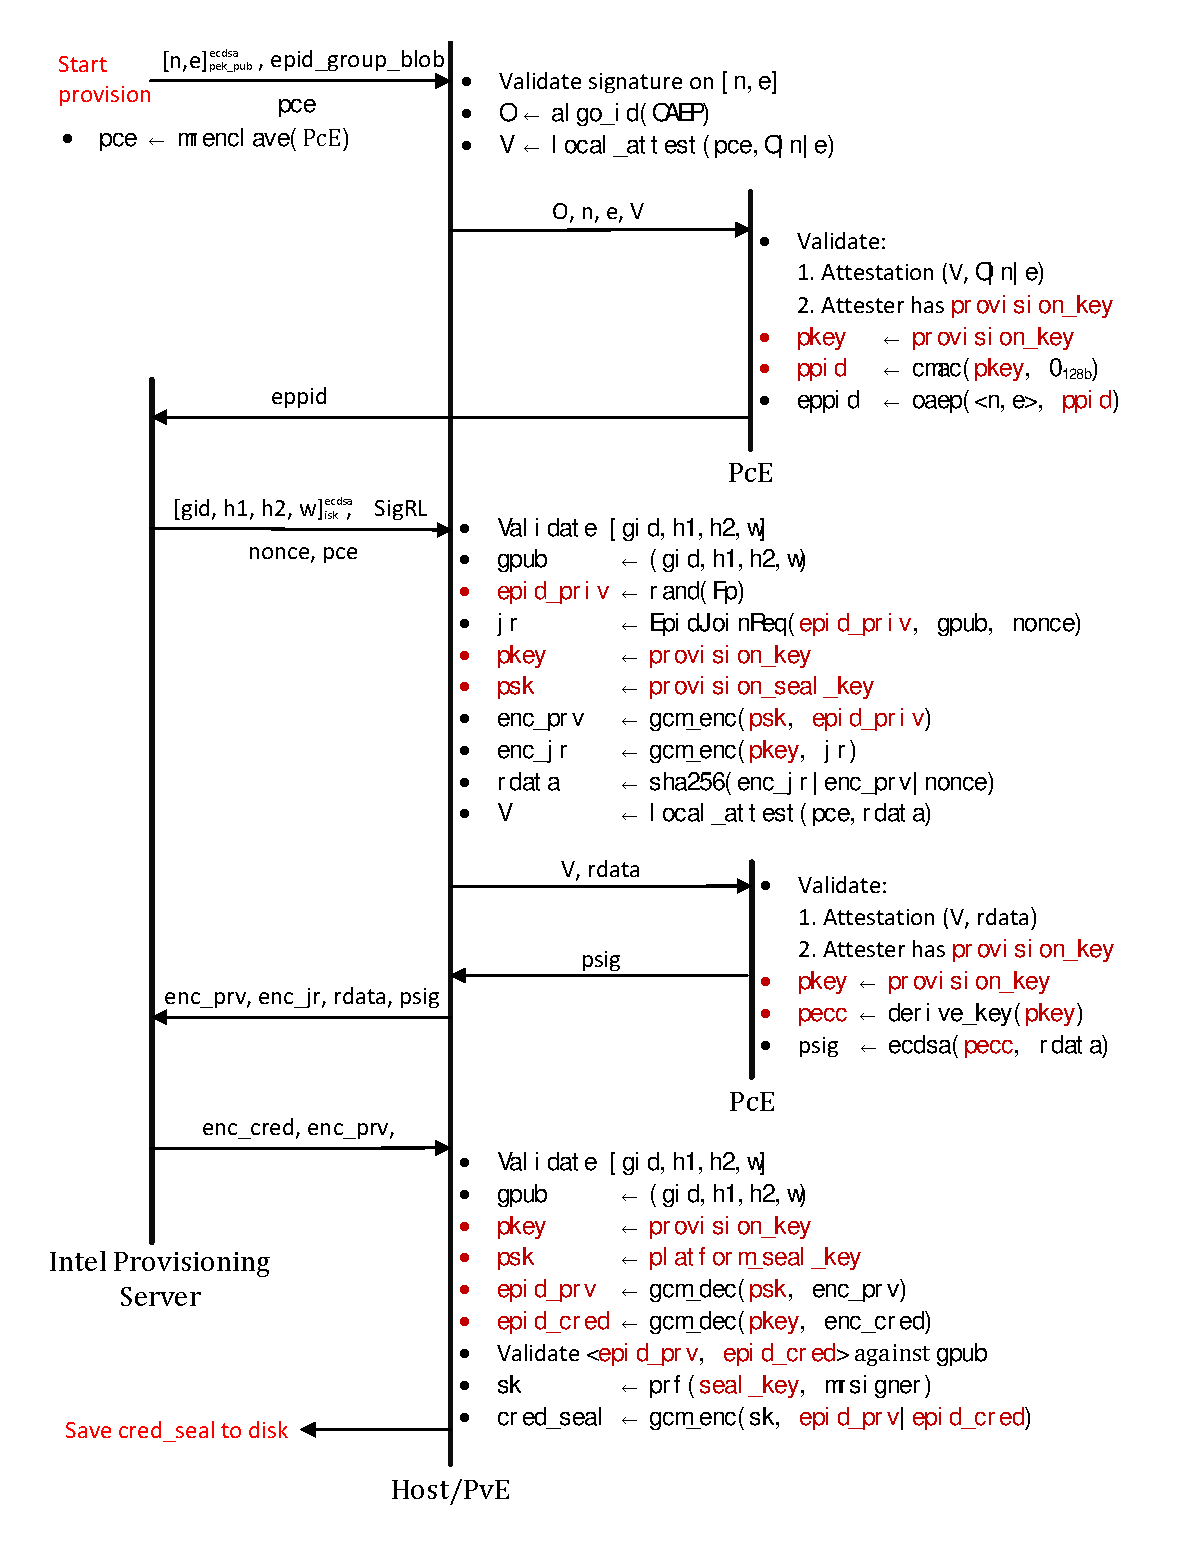
\includegraphics[width=0.8\linewidth]{Diagrams/EpidProvisioning}
  \caption{EPID Provisioning}
  \label{fig:epidprov}
  \end{figure}

  As described in \secref{sec:remoteatt}, each SGX capable processor
  has a unique Provisioning Key that's also known to Intel Attestation
  Service. In theory, one could use this key as the private key (the
  $\gamma$ in \cite{epid}) for EPID signatures. There are two problems
  with this: First a compromise of this key would render the CPU
  useless in-perpetuity. But more importantly, since EPID does not
  have full-anonymity and Intel knows this key, the scheme will lose
  anonymity.

  In order to create new set of EPID credentials, the SGX capable
  processor must participate in the EPID Join processor. When
  presented with a join request, the Intel Attestation Service must
  somehow ensure that the join request indeed came from an SGX
  processor; allowing non-SGX platforms to join SGX EPID group would
  render the entire remote attestation scheme useless. To make matters
  worse, under concurrent composition, the Zero-Knowledge Proof of
  Knowledge Protocol used in the EPID Join request is not secure, and
  the entity making the Join request (namely, \pve) must somehow
  ensure sequential execution.

  Intel has addressed these issues by creating two Intel signed
  enclaves called \pve\ and \pce\footnote{While we not sure why the
    provisioning process was split into two separate enclave with the
    same set of privileges, we believe this is done to separate the
    enclave that directly interacts with network data (\pve) from the
    one that only signs (certifies) messages.}. Both these enclaves
  have access to the Provisioning Key, and the \mrsigner\ for these
  enclaves is hard-coded in the \launchenclave---preventing non-Intel
  enclaves from gaining access to the Provisioning Key.

  Figure~\ref{ssec:epidprov} describes the details about EPID
  provisioning.
 
\bibliographystyle{alpha} \bibliography{sgx_biblio}
\end{document}
\documentclass[letterpaper]{article} \usepackage{cite}
\usepackage{amsfonts} \usepackage{fancyhdr}
\usepackage[svgnames]{xcolor} \usepackage[colorlinks=true,
  urlcolor=black!65!white, linkcolor=black!65!white,
  urlcolor=black!65!white, citecolor=black!65!white ]{hyperref}
\usepackage{url} \usepackage{tikz}
\usetikzlibrary{shapes,snakes,arrows} \usepackage{graphicx}
\usepackage{caption} \usepackage{subcaption} \usepackage{listings}
\usepackage[mono]{inconsolata}

\topmargin=-5mm \evensidemargin=0cm \oddsidemargin=0cm \textwidth=16cm
\textheight=22cm \addtolength{\headheight}{1.6pt}
\hypersetup{pdfstartview=}

\tikzset{>=latex}

\newcommand{\secref}[1]{\S\ref{#1}} \newcommand{\lastupdate}{\today}
\newcommand{\ie}{\textit{i.e.}}  \newcommand{\mdash}{---}
\newcommand{\ecall}{\textsf{ecall}}
\newcommand{\ocall}{\textsf{ocall}} \newcommand{\aex}{\textsf{AEX}}
\newcommand{\env}{\textsf{environment}}
\newcommand{\mrenclave}{\textsf{mrenclave}}
\newcommand{\mrsigner}{\textsf{mrsigner}}
\newcommand{\sha}{\textsf{sha256}} \newcommand{\pve}{\textsf{PvE}}
\newcommand{\pce}{\textsf{PcE}} \newcommand{\qe}{\textsf{QE}}
\newcommand{\launchenclave}{\textsf{Launch Enclave}}
\newcommand{\uc}{\textsf{UC}} \newcommand{\se}{source-enclave}
\newcommand{\te}{target-enclave} \newcommand{\rpk}{\textsf{Root
    Provisioning Key}} \newcommand{\pk}{\textsf{Provisioning Key}}
\newcommand{\psk}{\textsf{Provisioning Seal Key}}
\newcommand{\rsk}{\textsf{Root Seal Key}}
\newcommand{\sk}{\textsf{Seal Key}} \newcommand{\lk}{\textsf{Launch
    Key}} \newcommand{\rk}{\textsf{Report Key}}

\title{\bf Intel SGX Remote Attestation is not sufficient}
\author{\textsc{Yogesh Prem Swami}}

\date{\lastupdate}

\begin{document}
\pagenumbering{arabic}

\maketitle

\begin{abstract}
  Intel SGX enclaves provide hardware enforced confidentiality and
  integrity guarantees for running pure computations (\ie, OS-level
  side-effect-free code) in the cloud environment. In addition, SGX
  remote attestation enables enclaves to prove that a claimed enclave
  is indeed running inside a genuine SGX hardware and not some
  (adversary controlled) SGX simulator.

  Since cryptographic protocols do not compose well
  \cite{cramerthesis,ucframework,gnuc}, especially when run
  concurrently, SGX remote attestation is only a necessary
  pre-condition for securely instantiating an enclave. In practice,
  one needs to analyze all the different interacting enclaves as a
  single protocol and make sure that no sub-computation of the
  protocol can be simulated outside of the enclave. In this paper we
  describe protocol design problems under (a) sequential-composition,
  (b) concurrent-composition, and (c) enclave state malleability that
  must be taken into account while designing new enclaves. We analyze
  Intel provided EPID \cite{epid} \textsf{Provisioning} and
  \textsf{Quoting} enclave \cite{sgxattest} within this framework and
  report our (largely positive) findings. We also provide details
  about SGX's use of EPID and report (largely negative) results about
  claimed anonymity guarantees.

\end{abstract}

\section{Introduction}
\label{sec:intro}
  Intel SGX enclaves\cite{sgxinnov, sgxinnov2} provide hardware
  enforced confidentiality and integrity guarantees for running pure
  computation (\textit{i.e.}, OS-level side-effect-free code) in the
  cloud environment. By limiting the application's Trusted Computing
  Base (TCB) to the CPU and CPU-Cache, SGX provides unprecedented
  confidentiality and integrity guarantees against malicious OS
  kernels and supervisor software. A popular design methodology---as
  evidenced by \cite{Haven, Graphene, Scone}---for creating secure
  cloud applications is as follows:

  \begin{description}
    \item[Step-1:] First, define a remote-attestation mechanism to
      securely instantiate an enclave. Quite often, this step is not
      explicitly stated probably because a generic black-box
      attestation scheme---whatever that means---is expected to be
      sufficient.
    \item[Step-2:] Then, largely independently of the
      remote-attestation mechanism, define the functionality that
      needs to be implemented inside the enclave. This step often
      involves composing different cryptographic as well as
      non-cryptographic protocols in ad-hoc ways to implement the
      desired algorithm. For example, the enclave may need to read
      encrypted keys from disk, compute a signature based on that key,
      create a new set of keys, etc.
    \item[Step-3:] Finally, define a ``run-time workflow," where one
      first validates the remote-attestation result, and then runs the
      algorithm implemented by the enclave. This step often requires
      multiple interactions with various other entities such as other
      enclaves, untrusted host software, trusted remote client
      software, and other cryptographic devices such as TPMs.
  \end{description}

  It's hard to argue against the simplicity and ease of implementation
  of such a modular software design. However, as pointed out in
  \cite{ucframework, cramerthesis}, unless a protocol is designed for
  ``\textsf{Universal Composition}" (\uc)---where, the real-world
  behavior and the ideal-world definition (function) of a protocol are
  computationally indistinguishable \textit{for every} adversary
  controlled environment---it's unlikely that arbitrary composition of
  such protocols will be secure. On the other hand, proving results in
  the \uc-framework is rather difficult. In this paper we propose a
  framework for analyzing SGX enclaves that's a compromise between a
  full \uc-based analysis and completely ad-hoc composition. Before
  describing the framework, we illustrate the problem associated with
  the protocol composition with two real-world examples.

  To set the stage, a cloud service provider wanted to migrate its new
  clients from Amazon Cloud-HSM to an SGX enclave. The protocol for
  interacting with the enclave was based on HTTP Request/Response
  framework, where different operations (such as \textsf{KeyGen}),
  were sent as a command, and the enclave would execute and return a
  response (including explicit error codes) back to the remote caller.
  Important use-case for the enclave were to support (a) local key
  generation, (b) storing the public/private key on disk with an AEAD
  scheme that would allow \textit{fast} key look-up, and (c) creating
  Certificate Signing Requests (CSR) from the enclave using
  challenge-response protocol \cite[\S5.2.8.3]{rfc4210}, among other
  things. Figure~\ref{fig:sequentialcomp} describes one execution path
  of the protocol.

  \begin{figure}[h]
  \centering
  \begin{subfigure}[b]{.5\textwidth}
    \centering
    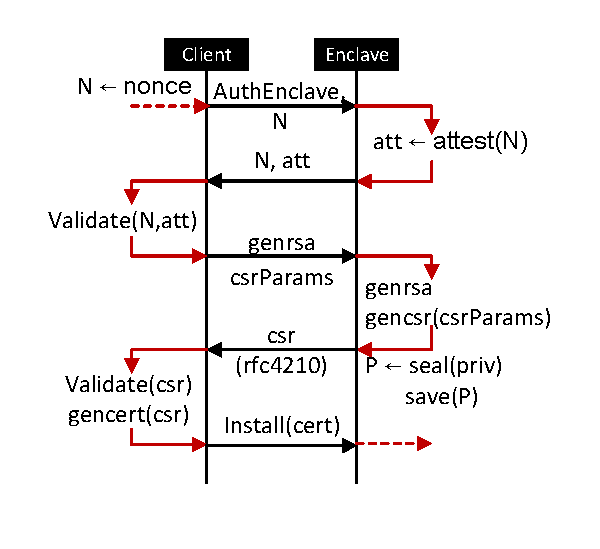
\includegraphics[width=.95\linewidth]{Diagrams/SeqCompProblem}
    \caption{Command execution for \textsf{KeyGen} with Cert}
    \label{fig:sequentialcomp}
  \end{subfigure}%
  \begin{subfigure}[b]{.5\textwidth}
    \centering
    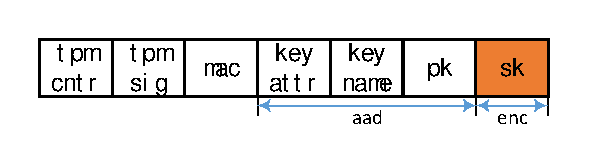
\includegraphics[width=.95\linewidth]{Diagrams/MsgFmt}\\\vfill
    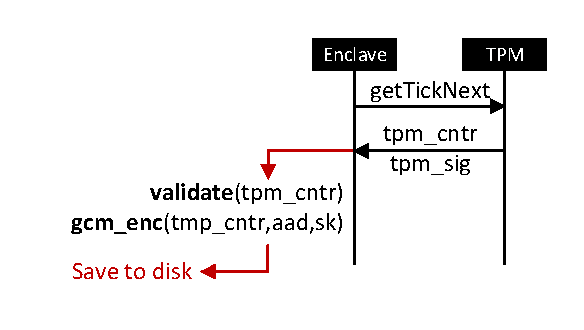
\includegraphics[width=.95\linewidth]{Diagrams/SealProtocol}
    \caption{Message format and seal protocol}
    \label{fig:sealprotocol}
  \end{subfigure}
  \caption{Example of a flawed key-management enclave. The command
    execution protocol ascertains the authenticity of the enclave by
    validating the EPID signature on a randomly generated 256-bit
    nonce, followed by executing an arbitrary mix of commands as
    required by the use-case. Long-term keys are stored as
    GCM-encrypted AEAD blobs. The nonce (a 32-bit counter zero-padded
    on the left to 96-bit) for each GCM record is stored in TPM, and
    the TPM returns a signature on the nonce (along with some
    additional data---to disable roll-back of TPM ``ticks.'' The
    enclave validates the TPM's signature before using the nonce for
    sealing.}
  \label{fig:usecase}
  \end{figure}

  This seemingly secure protocol is, in fact, not secure at
  all. Notice that the remote attestation in
  Figure~\ref{fig:sequentialcomp} does not prevent a malicious cloud
  service provider from first faithfully responding to remote
  attestation queries, but then emulate the rest of the protocol
  (including \textsf{KeyGen} and CSR) outside of the enclave. While
  this is obvious in this simplified example, in a more complicated
  scenario, where multiple enclaves are interacting with each other,
  it might not be obvious if certain sub-components of the protocol
  can be simulated outside. Even though the entire enclave is
  \textit{sequentially composed} from potentially provably-secure
  protocols, the combined protocol is completely insecure.

  Second, consider the seal protocol. Here each record (see
  Figure~\ref{fig:sealprotocol}) is GCM-encrypted using a nonce
  generated and signed by a TPM. However, consider a cloud service
  provider who instantiates two copies of the same enclave and
  \textit{concurrently} executes \textsf{KeyGen} using the same TPM
  signed counter. In this case, each enclave will generate two
  different keys in response to \textsf{KeyGen}. However, since the
  two concurrent instances will each correctly verify the signature
  (the two enclaves are identical), each will end up using the same
  nonce with different underlying data! As is the case with all
  counter modes, reusing the nonce can completely destroy the security
  of the system\footnote{In the present case, since the underlying
    data is uniformly distributed, at least for AES or ECDSA keys,
    such a concurrent composition might not be harmful. However, if
    there is even a small bias in the random number generator, it
    might be possible to build a distinguisher from the \texttt{xor}
    of cipher-text data.}. Note that this is not a flaw in GCM or in
  the way the TPM is used\footnote{When using TPMs with SGX enclaves,
    it's important that both the TPM and the enclave mutually
    authenticate each other. Failure to do so can lead to replay
    attacks where the adversary swaps the motherboard and in doing so
    resets the TPM counter. In the present case, however, even
    mutually authenticated TPM counter might not be secure under
    concurrent composition.}, rather, it's a case where an otherwise
  secure protocol is insecure under concurrent composition.

  While these examples describe a totally broken scheme, in practice
  sequential and concurrent composition may not completely break the
  system as above. Rather it might just weaken the \textit{bounds} of
  the entire protocol making it easy for further crypt-analysis. For
  example, consider a scheme that consists of to two protocols $\pi_1$
  and $\pi_2$, where the adversary needs $2^{t_1}$ and $2^{t_2}$
  oracle queries to break $\pi_1$ and $\pi_2$ respectively. However,
  its possible that when composed sequentially as $\pi_1 \circ \pi_2$
  or $\pi_2 \circ \pi_1$ the number of queries needed to break the
  composed protocol is smaller than $2^{\min\{t_1,t_2\}}$. In fact,
  since protocol composition rarely commutes, even different order of
  composition might result in very different bounds\footnote{Readers
    familiar with \textsf{encrypt-then-mac} vs.
    \textsf{mac-then-encrypt} debate should require no further
    explanation.}.
  
  To summarize, \textit{an enclave is a protocol} composed of several
  sub-protocols. In order for the enclave to be secure, it's essential
  that sequential and concurrent composition of sub-protocols remain
  secure. The rest of this document is organized as follows.
  \secref{sec:model} describes the abstract computational model of SGX
  that's better suited for security analysis. \secref{sec:analysisfwk}
  describes pitfalls of sequential, concurrent, and parallel
  composition of cryptographic protocols and describes ways in which
  an enclave can be abused by a malicious cloud service
  provider. \secref{sec:remoteatt} describes Intel's remote
  attestation framework, and describes in detail the SGX remote
  attestation mechanism.

  \section{SGX Computational Model}
  \label{sec:model}
  Intel documentation\cite{intelsdm} provides excellent low-level
  details about the SGX instructions. This section provides an
  abstract computational model of SGX which is better suited for
  security analysis.

  Abstractly, an SGX enclave can be thought of as a black-box that's
  capable of running any arbitrary algorithm. The black-box (enclave)
  can communicate with the outside world, called the \env, in three
  different ways:

  \begin{figure}[h]
  \centering 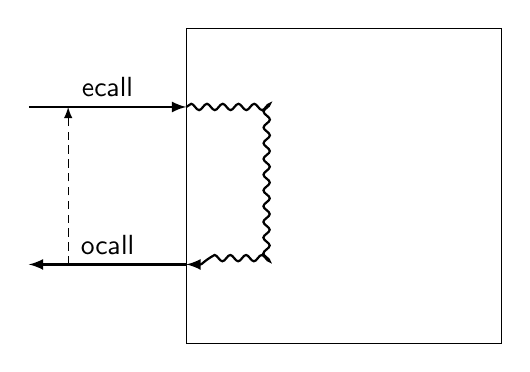
\begin{tikzpicture}[x=1cm, y=-1cm]
  \newcommand{\ench}{4cm}
  \newcommand{\encw}{4cm}
  \newcommand{\alen}{1cm}
  \newcommand{\adiff}{1cm}

  \node[rectangle, minimum height=\ench, minimum width=\encw, draw] (enc) {};
  \draw[->,thick] (-\encw / 2.0 - 2*\alen, \adiff ) -- (-\encw/2.0, \adiff) %%
  node [midway, above] {\textsf{ecall}};

  \draw [->, thick, decorate, %%
    decoration={snake,amplitude=.4mm,segment length=2mm, post length=1mm}] %%
  (-\encw/2.0, \adiff) -- (-\encw/2.0 + 1*\adiff + 0.1, \adiff) -- %%
  (-\encw/2.0 + 1*\adiff , -\adiff) -- (-\encw/2.0, -\adiff);


  \draw[<-,thick] (-\encw / 2.0 - 2*\alen, -\adiff ) -- (-\encw/2.0, -\adiff) %%
  node [midway, above] {\textsf{ocall}};

  \draw[->, thin,densely dashed] (-\encw / 2.0 - 1.5*\alen, -\adiff ) -- %%
  (-\encw/2.0 - 1.5*\alen , \adiff);
\end{tikzpicture}

  \caption{SGX Computational Model.}
  \label{fig:model}
  \end{figure}

  \begin{description}
  \item[\ecall:] The \env\ can invoke a pre-defined function inside
    the enclave by passing input parameters and returning internal
    state of the enclave as results. Such invocations from the
    \env\ to the enclave are referred to as \ecall. The parameter
    values passed from the \env\ to the enclave are either copied or
    directly shared with the enclave. An \ecall\ can terminate in one
    of the three ways: (a) by returning normally as a function from
    the enclave, (b) by making an explicit \ocall, or (c) as the
    result of an interrupt or exception.

    SGX also supports multi-threading, and it's possible for the
    \env\ to run the same \ecall\ in different threads. However, once
    an \ecall\ has acquired the thread, future attempts to reuse that
    same thread will result in error. Further more, the number of
    threads that an enclave can support is pre-determined by the
    enclave signer, and cannot be altered at runtime.

  \item [\ocall:] While an enclave is executing (because of some
    previous \ecall), it can make \ocall s to pre-designated functions
    in the \env.  Unlike an \ecall, an \ocall\ cannot directly share
    the internal enclave state with the \env, and must---directly or
    indirectly---copy the parameters into the \env\ before making an
    \ocall.

    An interesting characteristic of an \ocall\ is that the \env\ is
    not required to return back to the enclave at the end of the
    \ocall\ (see Figure~\ref{fig:model}). Since the behavior of
    pre-designated functions in the \env\ are controlled by the
    adversary, one should not expect the \env\ to follow the protocol
    that enclave author had envisioned. In particular, it's possible
    to create a chain of \ecall s and \ocall s such that the adversary
    can perform operations on the internal (global) state of the
    enclave. We call such adversarial manipulation of internal enclave
    state as \textit{enclave malleability}.

  \item[\textsf{Asynchronous Exit}:] In addition to an \ocall, the
    processor can exit from an enclave due to an interrupt or
    exception. Such enclave exiting events are called
    \textsf{Asynchronous Exit Events}, or \aex. Unlike an \ocall, an
    \aex\ can transfer control from the enclave to the \env\ at
    arbitrary (possibly adversary controlled) points inside the
    enclave. Like \ocall s, an \aex\ can either by resumed from where
    the enclave left off, or the environment can invoke another
    \ecall\ (either within the same thread or a different thread).

    Since an adversary can create multiple running copies of an
    enclave and selectively interrupt each enclave to cause and \aex,
    it can be used as a means to ``rewind'' the internal state of the
    enclave. Given that proof-of-knowledge \cite{BellarePOK} protocols
    fundamentally have a \textit{knowledge-extractor} based on
    rewinding, an enclave must ensure that it does not leak secrets
    when interrupted by an \aex.

  \end{description}

  \subsection{Enclave Creation}
  \label{sec:enclavecreateion}
  An enclave is generated as a dynamically shared library using
  standard compiler tools. In addition, the entity creating the
  enclave must also decide up-front on the following information:

  \begin{description}
  \item[\textsf{Attributes}:] The attributes of an enclave act as an
    access control mechanism that is enforced by the hardware. For
    example, certain high privilege keys, such as \lk\ and
    \textsf{Provisioning Key}, cannot be made accessible to all the
    enclaves, as it would compromise the security of entire SGX
    ecosystem. In order to gain access to these keys, an enclave
    author must explicitly request for these attributes at
    compile/sign time. During enclave launch-time, the \launchenclave,
    based on policy decisions, decides whether to grant or reject
    requests based on these attributes.

  \item[\textsf{Stack size}:] The enclave author must estimate the
    size of the stack needed by the enclave and set its value at
    enclave creation time. Once an enclave is instantiated, this value
    cannot be changed.

  \item[\textsf{Heap size}:] Like the stack size, the heap-size of the
    enclave is also fixed at enclave creation time. In SGXv2, this
    value can be changed post-instantiation.

  \item[\textsf{Thread count}:] An enclave must also decide upon the
    number of threads that can run concurrently. As pointed out in
    \secref{sec:model}, concurrency can have a dramatically negative
    impact on the security of the certain protocols, and one must not
    select this parameter just on the basis of performance
    requirements, but also on the basis of security concerns.

  \item[\textsf{Software version}:] SGX provides elaborate
    software-upgrade and life-cycle management facilities and allows
    software vendors to make use of these features.

  \end{description}

  Based on these parameters, the enclave signing tool creates a
  virtual memory layout of the enclave and computes a hash of the
  entire memory layout (including the stack, heap, thread control
  structure, etc.)  See \cite{intelsdm} for details about how the hash
  is computed. This hash, called \mrenclave, is used as the unique
  identifier for the enclave.

  In addition to \mrenclave, the software vendor must also sign the
  enclave using a RSA-3072 key. The hash of the RSA Public-Key is
  called \mrsigner. As described in \cite{surnaming}, the purpose of
  the signature is to provide an unforgeable identity---a
  \textit{surname} based lineage---to a set of enclaves based on the
  vendor.

  It should be noted that the \mrenclave\ of an enclave doesn't change
  even when the signing key is changed. This is significant when
  validating attestation or deriving keys based on \mrenclave.

  \subsection{Enclave instantiation and access control}

  A properly signed enclave can be instantiated on any Intel SGX
  Processor---subject to access control restrictions enforced by
  \launchenclave. Before an enclave can be instantiated on an SGX
  capable processor, it must get an authorization token, called
  \textsf{Launch Token}, from Intel provided \launchenclave. The
  \launchenclave\ uses a combination of \mrenclave, \mrsigner, the
  attributes of the enclave and a \textit{white-list signed by Intel}
  to decide whether to grant \textsf{Launch Token} to the enclave or
  not. Once an enclave obtains a \textsf{Launch Token}, the enclave
  can continue using it indefinitely, even when the policies of the
  \launchenclave\ might get updated later on.

  \subsection{SGX Platform Keys}
  \label{ssec:platkeys}

  As described in \cite{sgxattest}, each Intel SGX capable processor
  contains two statistically independent base keys: \rpk\ and \rsk.
  The \rpk\ is used as the \textit{root-of-trust} between the CPU and
  Intel Attestation Services (IAS) \cite{ias}. Intel retains a copy of
  this key at the time of manufacturing and uses it to establish the
  trustworthiness of the processor during EPID join process. Intel
  claims that \rsk\ is not retained. However, it's not clear whether
  this key is generated inside the processor via oracle access (\ie,
  in such a way that CPU generates the key all by itself using it's
  own internal random numbers or with PUFs), or whether the key is
  first generated outside the processor, then injected into CPU, and
  finally all outside references destroyed. Unless these keys are
  generated via oracle access, one should consider \rsk\ to be known
  to Intel.

  \begin{figure}
  \centering
  \begin{subfigure}[t]{.45\textwidth}
    \centering
    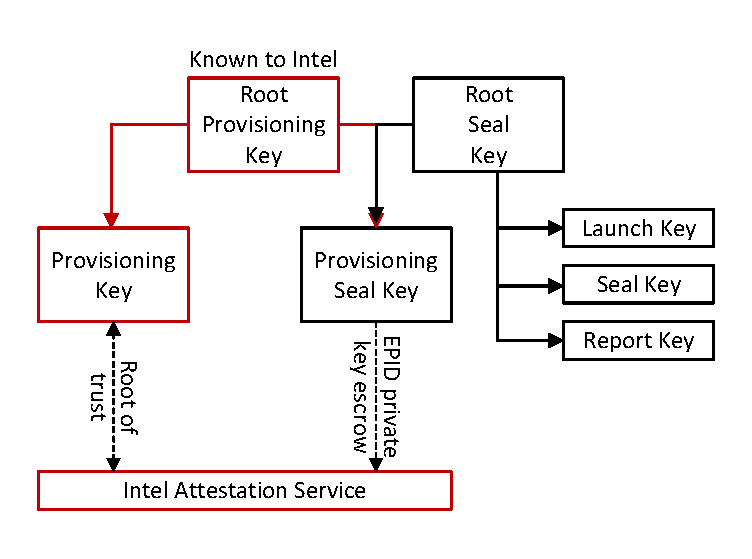
\includegraphics[width=\linewidth]{Diagrams/KeyHierarchy}
    \caption{The \pk\ acts as a root-of-trust between SGX capable CPU
      and Intel Attestation Service. \psk\ is used for EPID private
      key escrow.}
    \label{fig:keyhierarchy}
  \end{subfigure}
  \hspace{.05\textwidth}
  \begin{subfigure}[t]{.45\textwidth}
    \centering 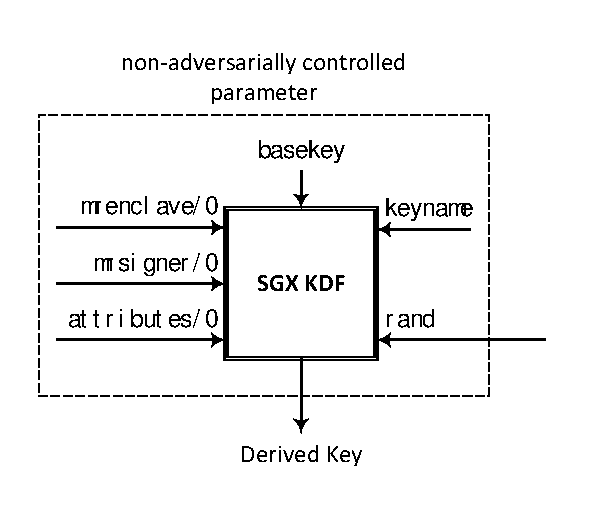
\includegraphics[width=\linewidth]{Diagrams/SGXKDF}
    \caption{SGX Key derivation function. Only parameters outside the
      dotted line can be chosen maliciously. Key derivation uses
      all-zeros for \mrenclave, \mrsigner, and attributes if key
      policy doesn't specify which ones to use. See
      \cite[\S38.17]{intelsdm} for additional details.}
    \label{fig:sgxkdf}
  \end{subfigure}
  \caption{SGX Platform and Named Key.}
  \label{fig:keys}
  \end{figure}

  An application software does not have raw access to these base
  keys. However, an application can access \textit{named} keys that
  are derived from these two base key (see Figure~\ref{fig:keys}).
  The key derivation function allows enclave author to specify
  policies on how to derive enclave specific keys from base
  keys. These policies allow enclaves to use the \mrenclave,
  \mrsigner\ and/or attributes from the trusted CPU cache to derive
  keys. An implication of this design is that enclaves cannot derive
  keys that might belong to a different enclave. Also note that when
  key derivation policy does not require specific field such as
  \mrenclave\ to be used, a default value of all-zeros is
  used. Therefore, even when ``raw'' named keys are available that
  have not been specialized for any particular enclave, it's not
  possible to derive specialized keys from the raw key. For example,
  one can obtain the raw \sk\ that is neither tied to \mrenclave\ or
  \mrsigner\ of any enclave, and yet it's not possible to derive
  enclave-specific \sk\ from the raw \sk.

  The following list describes user accessible keys and their intended
  usage:

  \begin{description}
  \item[\pk:] This key is derived from \rpk\ and is used as a software
    version dependent root-of-trust between Intel Attestation Service
    and SGX capable processor. Since admitting a non-SGX processor to
    the Intel Attestation Service's group of SGX processors will
    completely compromise remote attestation for all CPUs, extreme
    care must be taken in granting access to Provisioning
    Key. Currently, the \launchenclave\ only grants Provisioning Key
    access to enclaves that have been signed by Intel. Furthermore,
    only \textsf{Provisioning Enclave} (\pve) and Provisioning
    Certification Enclave (\pce) (both created without debug option)
    have access to this key.

  \item[\psk:] This key is derived jointly from Root Provisioning Key
    and Root Seal Key. During the EPID join process, the EPID
    private-key for each platform is encrypted with this key and
    uploaded to Intel Attestation Service. (See \secref{ssec:epidprov}
    for details about EPID join process.)

    Note that the EPID private-key could not just be encrypted with
    \pk\ as that would destroy the EPID's blinded-join
    protocol. Conversely, the EPID private-key cannot be encrypted
    just with \sk\ as that might allow non-privileged enclaves to have
    access to EPID private key and thereby render Remote Attestation
    ineffective.

    In spite of this design choice, given the uncertainty about how
    the \rsk\ is generated, one should assume that Intel knows the
    EPID private key for each platform.

  \item[\lk:] This key is derived from \rsk\ and is used by
    \launchenclave\ to create authorization tokens
    (\textsf{EINITTOKEN}) that each non-Intel enclave must obtain in
    order to instantiate an enclave. Only a specific \mrsigner---whose
    corresponding private-keys are only known to Intel---can access
    the \lk. In SGXv2, the \mrsigner\ for \launchenclave\ can be
    changed pragmatically, (see \cite[\S39.1.4]{intelsdm}) but it's
    not clear how Intel intends to enforce access control restrictions
    on \pk.

  \item[\sk:] This key is derived from \rsk\ and used for encrypting
    data specifically for a given CPU.

  \item[\rk:] This key is derived from \rsk\ and used for Local
    Attestation (see \secref{ssec:localatt} for detailed information
    on Local Attestation and how Report Key is used).

  \end{description}

  \subsection{Local Attestation}
  \label{ssec:localatt}

  \begin{figure}
    \centering
    \begin{subfigure}[h]{.5\textwidth}
      \centering
      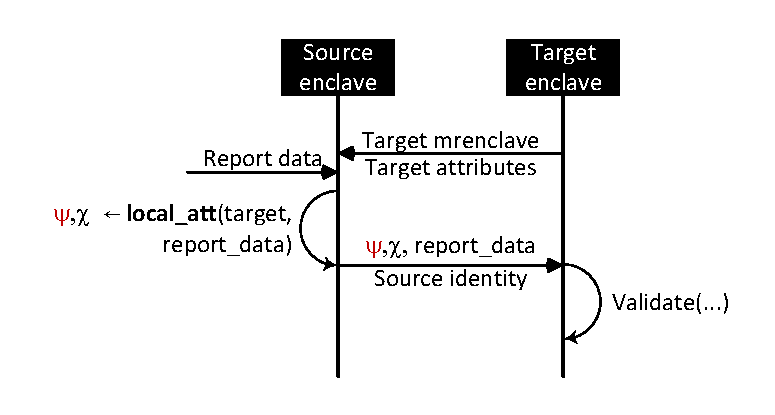
\includegraphics[width=.95\linewidth]{Diagrams/LocalAttestationFlow}
      \caption{Local attestation message flow.}
      \label{fig:localattestationflow}
    \end{subfigure}%
    \begin{subfigure}[h]{.5\textwidth}
      \centering
      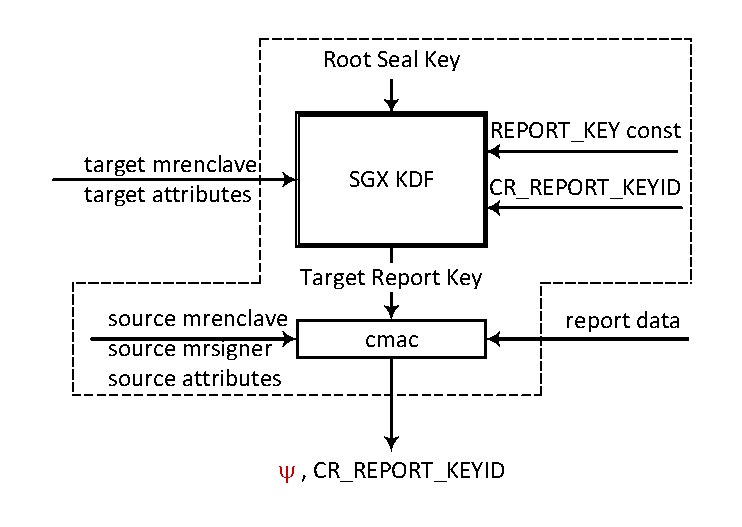
\includegraphics[width=.85\linewidth]{Diagrams/LocalAttestation}
      \caption{Local attestation computation. Parameters outside the
        dotted line can be adversarialy selected.}
      \label{fig:localattestation}
    \end{subfigure}%
    \caption{Local attestation computation and message flow}
    \label{fig:localatt}
  \end{figure}

  The process of local-attestation allows a source enclave (\se) to
  prove to a target enclave (\te)---running locally on the same
  platform---that the \se\ is indeed running on a genuine Intel SGX
  platform (see Figure~\ref{fig:localattestationflow}). In addition,
  the \se\ can optionally use 512-bits of additional data (e.g., hash
  of public-key), called report-data, to claim knowledge of certain
  bit-string.

  The process of local-attestation involves computing CMAC
  \cite{aescmac} on the \se's identity (i.e., \mrenclave, \mrsigner,
  etc.) using the \te's Report Key. However, as pointed out in
  \secref{ssec:platkeys}, the \se\ cannot directly access \te's Report
  Key. SGX solves this problem by providing \textit{oracle access} to
  \te's Report Key via \textsf{EREPORT} instruction
  \cite[\S14.4.1]{intelsdm}.
  
  To compute local attestation, the \se\ obtains the \mrenclave\ and
  attributes of the \te\ through some out-of-band mechanism (which
  might be adversarial). Based on \te's \mrenclave, the
  \textsf{EREPORT} instruction internally derives the \te's Report Key
  and computes \textsf{CMAC} on \se's \mrenclave, \mrsigner, and
  attributes from the trusted CPU cache (and optionally untrusted user
  data).  The \textsf{EREPORT} instruction also uses a boot-time
  random number called \textsf{CR\_REPORT\_KEYID} to diversify the
  \te's Report Key before \textsf{CMAC} computation. The
  \textsf{EREPORT} instruction also returns the value of
  \textsf{CR\_REPORT\_KEYID} that was used during \te's Report Key
  derivation.

  The verification of local attestation involves using
  \textsf{EGETKEY} instruction to fetch the \te's Report Key and
  validating the \textsf{CMAC} on Report body in software.  The report
  body includes \mrsigner, \mrenclave, attributes, and other
  parameters of the \se. Note that while fetching the \rk\ for
  verification, the \textsf{EGETKEY} will require the value of
  \textsf{CR\_REPORT\_KEYID} to derive the right \rk.

  \section{Enclave Malleability and Knowledge Extractors}
  \label{sec:analysisfwk}

  Given the computational model of SGX, we describe certain pitfalls
  in enclave design that might inadvertently make the enclave
  malleable, or open door for building knowledge-extractors
  \cite{BellarePOK}.

  \subsection{Enclave Malleability}
  \label{ssec:malleability}
  As described in \secref{sec:model}, an application can exit an
  enclave either via (a) as a function return from an \ecall\ (b) as
  an \ocall\ or (b) as an \aex. Since it's not required for an
  \ocall\ or \aex\ to return back to the enclave from the state it
  left off, it's possible for a malicious \env\ to make unexpected
  \ecall s to alter the internal state of the enclave. Enclaves whose
  global internal state can be influenced by an attacker by not
  following the expected protocol are called \textit{malleable
    enclaves} in this document.

  To better understand enclave malleability, consider the following
  example: The US government wants to use an SGX enclave to implement
  2-man rule for launching nuclear missiles. The 2-man rule requires
  that at least two \textit{different} members (generals) of the armed
  forces authorize the launch a nuclear missile.

  Listing~\ref{code:malleability} describes one way to implement this.
  Essentially, the enclave keeps a list of generals, their
  public-keys, and their individual authorization state in a global
  variable \texttt{GENERALS}. In addition, the enclave keeps the
  number of distinct generals who have authorized the launch in a
  global variable \texttt{auth\_count}. Since different generals might
  be authorizing the launch at different times, the enclave allows
  each general to authorize a launch individually by signing the
  concatenation of general's name and some auxiliary data.

  \begin{center}
  \lstset{language=C++, numbers=left, numberstyle=\tiny,
    numbersep=5pt, stepnumber=1, emph={auth_and_launch,auth_count},
    emphstyle=\color{red!80!black}, emph={[2]valid_general},
    emphstyle={[2]\color{green!40!black}}, basicstyle=\ttfamily,
    keywordstyle=\color{blue}\ttfamily,
    stringstyle=\color{red}\ttfamily,
    commentstyle=\color{brown}\ttfamily,
    morecomment=[l][\color{magenta}]{\#} }
  \begin{lstlisting}[captionpos=b,
                     caption={An enclave suseptible to state
                       malleability}, label=code:malleability] /*
    count of generals who have authorized launch. */ static int
    auth_count = 0;

/* hardcoded list of generals and their PKs */ struct general_info{
  char general_name[256]; const sgx_ec256_public_t general_pub; bool
  has_authorized; // initialized to false }GENERALS[] = { ... };

/* ecall made by each general with a sig on name + aux data */ int
auth_and_launch(const char* const general_name, const
sgx_ec256_signature_t* sig){ struct general_info* valid_general =
  validate_general(general_name, sig);

  if(!valid_general){ return INVALID_GENERAL; }

  if(!valid_general->has_authorized){ auth_count++; // \aex\ here will
    be devastating!  valid_general->has_authorized = true; }else{
    return GENERAL_ALREADY_AUTHORIZED_ACTION; // replay }

  if(auth_count == 2){ return nuke_the_kashbah(location); }

  return PENDING_AUTHORIZATION; }
\end{lstlisting}
\end{center}

  Can this enclave be exploited to launch a missile with \textit{just
    one} authorization, say $\langle g_1, \sigma_1 \rangle$?
  Surprisingly, the answer is yes! Here is how:

  \begin{enumerate}
  \item The attacker first feeds $\langle g_1, \sigma_1 \rangle$ to
    \texttt{auth\_and\_launch} function with the intent of causing an
    \aex\ between lines 19 and 20. Since the attacker can artificially
    cause an interrupt and also instantiate multiple copies of the
    enclave in parallel, given a polynomial number of trials (in
    program length), the attacker can cause an \aex\ between line 19
    and 20 W.H.P. Note that at the time of a successful \aex\ between
    line 19 and 20, the \texttt{auth\_count} and
    \texttt{has\_authorized} variables will be in an inconsistent
    state where the \texttt{has\_authorized} would still be
    \texttt{false} and another \ecall\ to \texttt{auth\_and\_launch}
    will successfully update the \texttt{auth\_count} variable.

  \item After the enclave has been interrupted by \aex\ and the
    processor is ready to resume, the attacker instead of resuming,
    makes an \ecall\ to \texttt{auth\_and\_launch} again with the same
    old parameters $\langle g_1, \sigma_1 \rangle$. Since the first
    \ecall\ had incremented the counter, but left the authorization
    state inconsistent, the second \ecall\ will once again increment
    \texttt{auth\_count} leading to a nuclear attack!

  \item While not applicable in this case, in some cases it might be
    necessary for an attacker to resume the first \ecall\ after the
    second one has completed. Since the enclave preserves the stack
    before making an \aex, resuming the first \ecall\ tantamounts to
    executing \textsf{ERESUME} assembly instruction.

  \end{enumerate}

  It should be emphasized that the problem of state-malleability,
  where the attacker can influence the internal state of the enclave
  without ever having direct authorized access to it, is broader in
  scope than the race condition described above. For example, one can
  use malleability to induce an error which turns the enclave into an
  oracle. It should also be emphasized that enclaves should return
  error codes with security consideration in mind.

  \subsection{Enclave rewinding and knowledge-extractors}
  \label{ssec:rewind}

  Zero-Knowledge Proof of Knowledge (ZKPK) protocols, by definition
  have in-built knowledge-extractor \cite{BellarePOK, maurerZKP}.
  Normally, the knowledge-extractor from the prover is designed by
  giving a simulator the capability to ``rewind'' the prover's state
  to arbitrary point during it's execution. Since SGX enclaves can be
  interrupted by an \aex, it's important that a malicious \env\ is not
  able to rewind the enclave in such a way that it inadvertently
  reveals the secret-key.

  Consider the three-move---commit, challenge,
  blinded-reveal---$\Sigma$-protocols \cite{sigmaprotocol} that are
  the most efficient and widely-used ZKPKs protocol in practice.
  Normally, one designs $\Sigma$-protocols \textit{with interaction}
  between a prover and a verifier in mind, and then uses Fiat-Shamir
  \cite{FiatShamir} heuristic\footnote{In the Fiat-Shamir heuristic,
    the prover \textit{pretends} to be a verifier and a random oracle,
    based on publicly known fields of the protocol (such as the
    commitment value, user's input message, etc.) generates the
    challenge string.} to convert it into a useful non-interactive
  use-case such as a signature scheme. Most of these protocols just
  require the prover, which in this case will be enclave, to respond
  to two challenge message for a given commitment message to reveal
  the secret.

  If an enclave is not implemented appropriately, one can induce an
  artificial \aex\ right after the commitment phase, and call the
  enclave with different messages in possibly different threads to
  generate two responses to the same commitment message. Note that
  \aex in conjunction with multi-threading opens doors for a limited
  form of enclave rewinding and presents a larger attack surface than
  \aex alone.  Unless, an enclave requires multi-threading, it's wise
  to set the number of possible threads to the bare minimum.

  \section{SGX remote attestation}
  \label{sec:remoteatt}

  SGX is an example of a hardware/software co-design of a
  cryptographic platform. A common concern in the design of such
  systems is to ensure that an adversary is not able to switch the
  hardware with a software simulator (such as QEMU \cite{qemu,
    opensgx}) of the hardware. Since an Universal Turing Machine can
  simulate any piece of computing hardware, unless there's an inbuilt
  asymmetry between what the software ``knows'' and what the hardware
  knows, it's impossible to prevent software simulator attacks in such
  systems. On the other hand, each independent piece of software needs
  to prove on its own that it's running on a real hardware.
  Therefore, each independent software must somehow have direct or
  oracle access to the secret that the hardware is holding. The
  essence of any remote-attestation scheme in such systems is to
  address these two conflicting requirements. {\em Note}: Even
  limiting access to raw hardware keys via an oracle is not sufficient
  to thwart simulator based attacks. An attacker can run it's hardware
  simulator on a real hardware, gain access to the hardware-secret via
  the oracle, and then impersonate as the real hardware.

  In case of Intel SGX, the question of knowledge-asymmetry between
  hardware and software is answered by the \rpk\ (see
  \secref{ssec:platkeys}). The dilemma of both denying as well as
  granting access to this hardware secret is solved by a two-step
  process:

  \begin{enumerate}
    \item Intel has created a (set of) privileged enclaves---called
      \textsf{Provisioning Enclave} (\pve) and \textsf{Provisioning
        Certification Enclave} (\pce)\footnote{Intel addresses these
        enclaves by their acronyms, \pve\ and \pce, only. The
        descriptive names are author's interpretation.}---with raw
      access to the Provisioning Key and Provisioning Seal Key. The
      \pve\ and \pce\ use the Provisioning Key as the root-of-trust
      between Intel Attestation Service and the SGX CPU to bootstrap a
      new set of credentials for a Group Signature Scheme called
      Enhanced Privacy ID (EPID) \cite{epid}. Since EPID key
      provisioning takes place only once\footnote{EPID re-provisioning
        might take place if the CPU's Security Version Number (CSVN
        \cite[\S39.4.2.2]{intelsdm}) or the Software Version Number
        (ISVSVN \cite[\S39.4.2.1]{intelsdm}) of \pce\ changes.}, the
      Provisioning Key has minimal exposure.

    \item Once a platform has been provisioned with EPID keys, another
      Intel signed enclave called \textsf{Quoting Enclave} (\qe) is
      given raw access to EPID keys and made responsible for
      generating remote-attestation results on behalf of other
      arbitrary--potentially malicious---enclaves.

      To compute remote attestation, an arbitrary enclave first
      generates a local attestation with \textsf{Quoting Enclave} as
      the target enclave in Figure~\ref{fig:localattestationflow}. The
      \textsf{Quoting Enclave} first validates the local-attestation
      report and subsequently uses EPID key to sign all the parameters
      it validated during local attestation. Since local-attestation
      uses the hardware resident identity of the enclave (i.e.,
      \mrenclave, \mrsigner, and enclave attributes), which cannot be
      forged (see \secref{ssec:localatt}), the remote-attestation
      result on the enclave identity cannot be forged
      either. Furthermore, since arbitrary software never has direct
      or oracle access to either Provisioning Key or EPID
      private-keys, simulator based attacks where the simulator itself
      is a valid enclave are also thwarted.
  \end{enumerate}

  The rest of this section is organized as follows: \secref{ssec:epid}
  provides an overview of EPID and how it's has been implemented by
  Intel. Since the official \cite{epid} paper leaves several details
  out (e.g., the Zero-Knowledge proof of inequality for signature
  based revocation is left out from the paper), the goal of this
  section to fill in those gaps based on \textsf{Provisioning Enclave}
  and \texttt{epid-sdk} open source implementation
  \cite{epidsdk}. \secref{ssec:epidprov} provides detailed information
  on how the \textsf{Provisioning Enclave} joins the SGX EPID
  group. Finally, \secref{ssec:qe} provides details about
  \textsf{Quoting Enclave} and how SGX remote attestation should be
  validated against Intel Attestation Service.

  \subsection{EPID Overview}
  \label{ssec:epid}
  In a standard signature scheme, such as ECDSA or RSA-PSS, each
  signer has a unique private/public key-pair. Given two
  message/signature pairs $\langle m_1, \sigma_1 \rangle$ and $\langle
  m_2, \sigma_2 \rangle$, an attacker in possession of $N$ public-keys
  can easily determine if $m_1$ and $m_2$ were signed by the same
  private key or not. If such signatures are generated by physical
  devices, it can be used to track the signing device and thereby
  destroy the anonymity and privacy of the person using that device.

  Group Signatures were introduced by Chaum and Van Heyst
  \cite{ChaumGroupSignatures} as a means to address this. Their idea
  was to create a signature-scheme where a single ``group
  public-key,'' can verify messages signed by different private
  keys. In addition to anonymity, several additional requirements were
  later on added to this list to different use cases.

  The literature on group signature schemes is huge, both for formal
  models of its security
  \cite{BMW03,dynamicGroupSignatures,fulldynamicgroupsignature} as
  well as for different constructions \cite{bbs, Furukawa2005,
    coalitionresistant, camenischLysyankaya} based on different
  computational assumptions. From a practical deployment perspective,
  Direct Anonymous Attestation \cite{daa, ucdaa} (DAA) is closest to
  EPID and also most widely deployed.


  In EPID, there are four entities:

  \begin{description}
  \item [Issuer ($\mathcal{I}$):] It's the entity that decides who
    should be part of a given EPID group. In case of SGX, the Intel
    Attestation Service acts as the issuer. Its goal is to dynamically
    (i.e., one-by-one) add new SGX Processors as they come
    on-line. Group signature schemes do no define what credentials one
    must possess before they can be admitted to given group. However,
    for group signatures to be meaningful, some form of out-of-band
    mechanism must decide group membership criteria. In case of SGX,
    the Intel Attestation Service uses knowledge of Root Provisioning
    Key as the deciding factor on who should join the SGX Processor
    group (see \secref{ssec:epidprov}).

  \item[Revocation Manager ($\mathcal{R}$):] Unlike standard signature
    schemes, where revocation only includes the public-key of the
    revoked private-key, group signatures require a different
    approach. EPID has two forms of revocation:

    \begin{itemize}
    \item Private-key based revocation list, called \texttt{Priv-RL},
      which is a list of all the compromised \textit{private-keys}
      known to Revocation Manager. EPID does not support
      full-anonymity\footnote{In the \textsf{anonymity} game of
        \cite{BMW03}, the adversary gets the private key of all the
        members, and yet cannot distinguish one signer from another
        based on signatures alone.} in the sense of \cite{BMW03}, and
      putting a private key in \texttt{Priv-RL}, completely destroys
      the anonymity of the signer.
      \item Signature based revocation, called \texttt{Sig-RL}, which
        is a list of message, signature pairs $\langle m_i, \sigma_i
        \rangle$ that the Revocation Manager believes to have been
        created by a fraudulent signer. Signature based revocation is
        an alternative to traceability found in most group signature
        schemes.
    \end{itemize}

    In EPID, a signer needs to have access to the most up-to-date
    \texttt{Sig-RL} to generate a valid signature. This is
    fundamentally different from \textit{verifier local revocation}
    (VLR) \cite{BonehVLR} where the signer never needs up-to-date
    revocation list to generate a valid signature. Also, unlike
    verifier local signatures, EPID signatures are of variable length
    and even same message signed with the same private-key can have
    different lengths depending upon the length of
    \texttt{Sig-RL}. It's surprising that such a signature scheme is
    can still be anonymous!

    \item[Platforms ($\mathcal{P}$):] Platforms in EPID are entities
      that are part of the signing group. In case of SGX, each SGX
      capable CPU SoC is a platform. Note that the issuer is not part
      of the Platform, and cannot create valid signatures on behalf of
      the group.

      Platforms generate their private key (essentially a group
      element in $\mathbb{F}_p^{\times}$) using a private-coin
      protocol. Through a \textit{blinded join} process, the Issuer
      grants a ``certificate'' on Platform's private key, which
      includes the group's identity as well as group
      public-key. Together, the Issuer certificate and Platform's
      private key form the platform signing key. In case of SGX, the
      \textsf{Provisioning Enclave} is responsible for joining the SGX
      EPID group. Once \textsf{Provisioning Enclave} has obtained a
      signing key from Intel Attestation Service, it stores this key
      on non-volatile storage encrypted with \sk\ that has been
      diversified using the \mrsigner\ of \pve. Since Intel is the
      \mrsigner\ of \pve, only Intel Signed enclave can access the
      EPID signing key.

      In order to sign a message, a platform needs access to its
      signing key and the recent most \texttt{Sig-Rl}.

    \item [Verifiers ($\mathcal{V}$):] Any entity in possession of the
      Group public-key is a verifier. In case of Intel Attestation
      Service, however, each signature is encrypted by the
      \textsf{Quoting Enclave} using an authenticated public-key in
      the enclave. The motivation for this is unclear, and currently
      only Intel Attestation Service can verify signatures.

      Note that not having the ability to verify signatures locally
      means that one must trust Intel Attestation Service with the
      validity of the signature. If Intel, for what ever reason,
      chooses to lie about the validity of a signature, it could
      completely compromise the security of the system.
  \end{description}

  Because of space and time constraints, we intentionally leave out
  additional details about EPID in the rest of the document. Since the
  EPID paper leaves out details about zero-knowledge proof of
  inequality of two discrete logs to make use of \texttt{Sig-RL}, we
  point that the SGX implementation uses \cite[\S6]{ShoupVFE} verbatim
  to achieve this.

  \subsection{SGX EPID provisioning}
  \label{ssec:epidprov}
  \begin{figure}
  \centering
  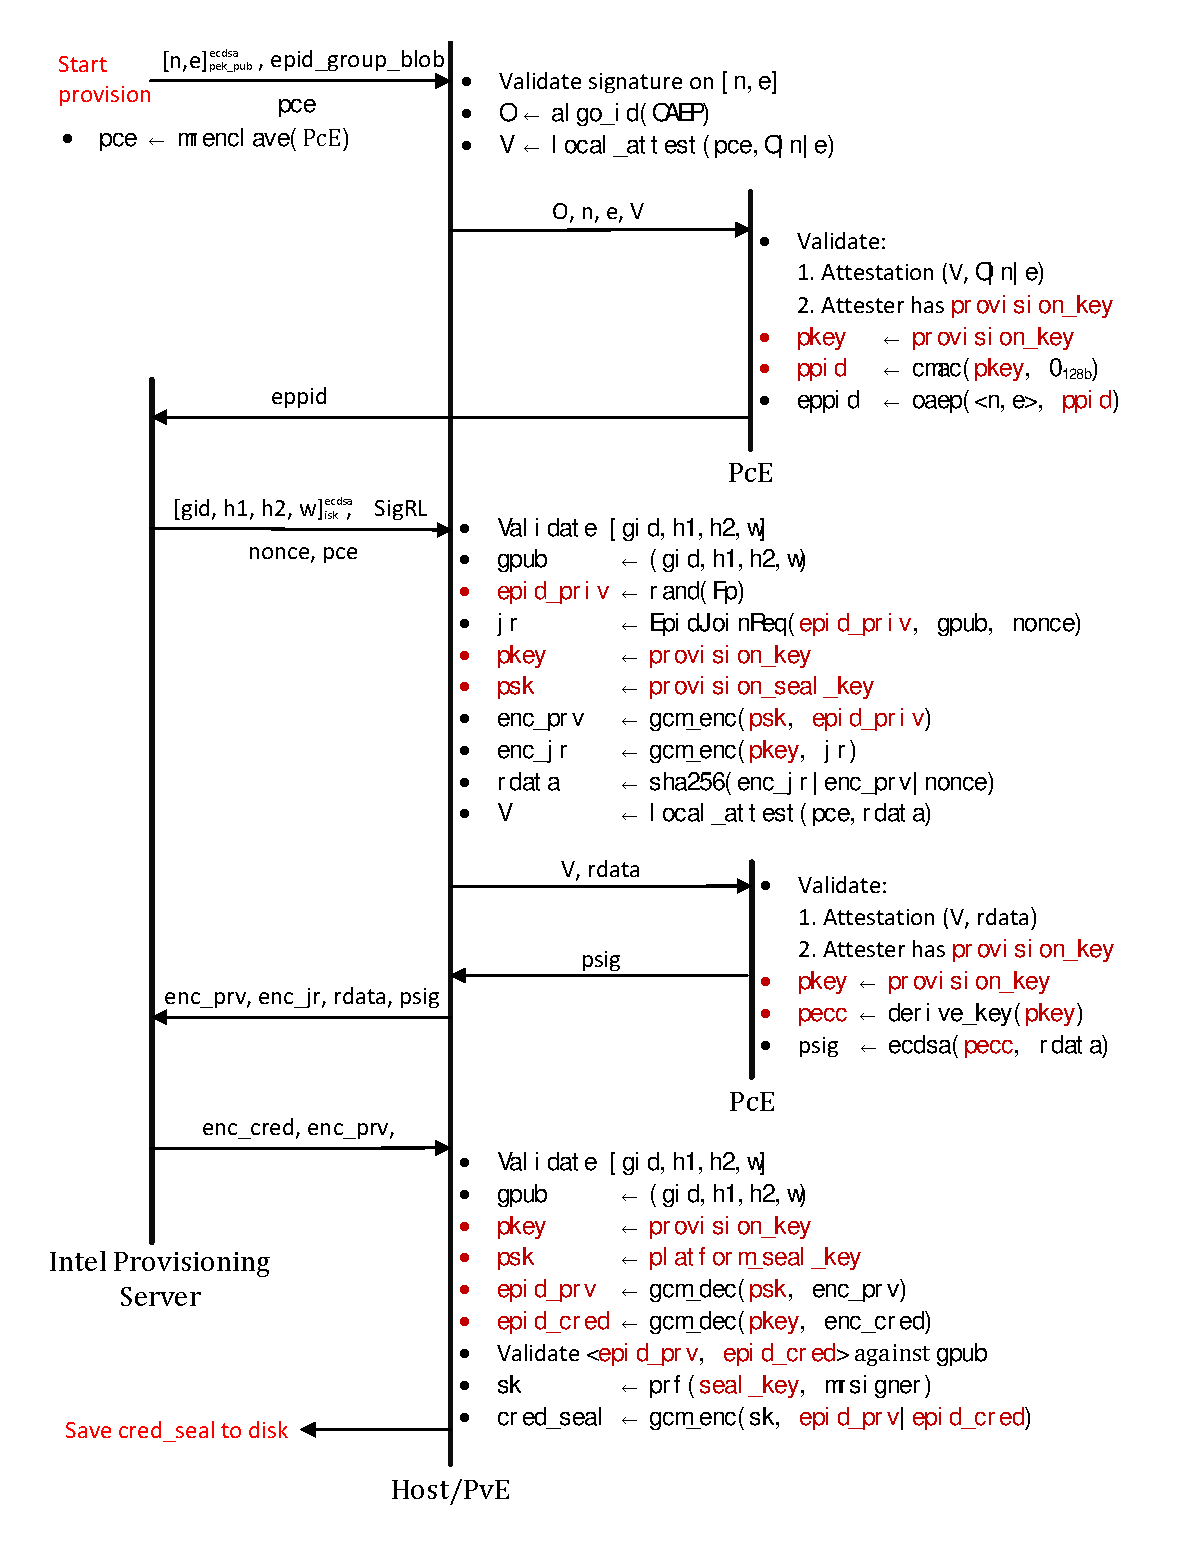
\includegraphics[width=0.8\linewidth]{Diagrams/EpidProvisioning}
  \caption{EPID Provisioning}
  \label{fig:epidprov}
  \end{figure}

  As described in \secref{sec:remoteatt}, each SGX capable processor
  has a unique Provisioning Key that's also known to Intel Attestation
  Service. In theory, one could use this key as the private key (the
  $\gamma$ in \cite{epid}) for EPID signatures. There are two problems
  with this: First a compromise of this key would render the CPU
  useless in-perpetuity. But more importantly, since EPID does not
  have full-anonymity and Intel knows this key, the scheme will lose
  anonymity.

  In order to create new set of EPID credentials, the SGX capable
  processor must participate in the EPID Join processor. When
  presented with a join request, the Intel Attestation Service must
  somehow ensure that the join request indeed came from an SGX
  processor; allowing non-SGX platforms to join SGX EPID group would
  render the entire remote attestation scheme useless. To make matters
  worse, under concurrent composition, the Zero-Knowledge Proof of
  Knowledge Protocol used in the EPID Join request is not secure, and
  the entity making the Join request (namely, \pve) must somehow
  ensure sequential execution.

  Intel has addressed these issues by creating two Intel signed
  enclaves called \pve\ and \pce\footnote{While we not sure why the
    provisioning process was split into two separate enclave with the
    same set of privileges, we believe this is done to separate the
    enclave that directly interacts with network data (\pve) from the
    one that only signs (certifies) messages.}. Both these enclaves
  have access to the Provisioning Key, and the \mrsigner\ for these
  enclaves is hard-coded in the \launchenclave---preventing non-Intel
  enclaves from gaining access to the Provisioning Key.

  Figure~\ref{ssec:epidprov} describes the details about EPID
  provisioning.
 
\bibliographystyle{alpha} \bibliography{sgx_biblio}
\end{document}
